\chapter{確率}

{\small この章を学ぶには, これまでの章(特に集合, 微分, 積分)を既に習得している必要があります。\\}

\section{事象}

「サイコロを1回投げる」という操作を考えよう。この操作は, 結果として, 「3(の目)が出る」
とか「偶数が出る」とか「4以上が出る」等のことが起きる可能性がある。しかし, 実際にこれらが起きるか
どうかは, やってみなければわからない。

この「サイコロを投げる」というような, やってみなければ結果
はわからないような\textgt{動作}(操作)を\underline{試行} (trial)と呼ぶ。そして, 
「3が出る」「偶数が出る」のように試行の結果として起きる可能性のあるできごとを
\underline{事象} \index{じしょう@事象} (event)と言う(確率事象とも言う)。

\begin{faq}{\small\textgt{試行とは何か? と問われて,「やってみなければわからないこと」と答えたら, 
正解をもらえませんでした。なぜ?}
... その答えでは, 試行と事象をはっきり区別できないからです。「サイコロをふって
どの目が出るか」は試行, 「サイコロをふって3(の目)が出る」は事象。でも, 両方とも, 
「やってみなければわからないこと」です。「こと」が動作を意味するのか結果を
意味するのかわからないのです。}\end{faq}

\begin{faq}{\small\textgt{そんな誤解をする人がいるとは思えませんが。}
... 世の中にはいろんな人がいます。科学は, できるかぎり誤解されない(まぎらわしくない)
言葉遣いを心がけねばなりません。どんな表現についても, 「これを誤解する人がいるとしたら, どう誤解するだろう? 
それを防ぐには, もっと良い表現は無いだろうか?」と, 考えることが大切なのです。}\end{faq}

ある試行に対して「2つの事象$A$と$B$の少なくとも片方が起きる」という事象を$A$と$B$の\underline{和事象}と呼び, 
\begin{eqnarray}A\cup B\label{eq:sumset}\end{eqnarray}と書く($\cup$は「和集合」を
あらわす記号)。

\begin{exmpl}\label{exmpl:event01} 「サイコロを1回投げる」という試行に
対して, 「偶数が出る」という事象を$A$, 「4以上が出る」
という事象を$B$とする。$A\cup B$は, 「偶数または4以上の数が出る」
すなわち「2か4か5か6が出る」という事象である。(例おわり)\end{exmpl}

ある試行に対して「2つの事象$A$と$B$がともに起きる」という事象を$A$と$B$の\underline{積事象}と呼び, 
\begin{eqnarray}A\cap B\label{eq:prodset}\end{eqnarray}
と書く($\cap$は「積集合」をあらわす記号)。上の例\ref{exmpl:event01}の
事象$A$, $B$について$A\cap B$は, 「偶数かつ4以上が出る」すなわち「4か6が出る」という事象である。

ある試行に対して, ある事象$A$とある事象$B$が同時に発生することがないこと, つまり積事象が
\underline{空事象} \index{くうじしょう@空事象} (何も起きることがないという事象; $\varnothing$とあらわす)
となるようなこと, すなわち
\begin{eqnarray}
A\cap B=\varnothing\label{eq:stat_event_exclusive_def}
\end{eqnarray}
が成り立つ場合, $A$と$B$は互いに\underline{排反} \index{はいはん@排反} (exclusive)
である, という。例えば, 「サイコロを1回投げる」
という試行に対して, 「2が出る」という事象と「3が出る」という事象は互いに排反である。

他の複数の事象の和事象と考えることはできないような事象を
\underline{根元事象} \index{こんげんじしょう@根元事象}という。
例えば「サイコロを1回投げる」という試行に対して, 「1が出る」という事象は, 
根元事象である。同様に「2が出る」「3が出る」...「6が出る」は, 
いずれもそれぞれ根元事象である。空事象以外のどのような
事象も, 根元事象の和事象として表現できる。例えば「サイコロを1回投げる」
という試行に対して「偶数が出る」という事象$A$は, 
\begin{eqnarray*}
A=\text{「2が出る」} \cup \text{「4が出る」}\cup \text{「6が出る」}
\end{eqnarray*}
というように, 3つの根元事象の和事象として表現できる(従ってこの事象$A$は
根元事象ではない)。

ある試行に関する全ての根元事象の和事象を\underline{全事象}
と呼ぶ\footnote{標本空間とも言う。}。サイコロの例で言えば, 
全事象$U$とは\footnote{全事象は慣習的に$U$と書くことが多い。}, 
\begin{eqnarray*}
U=\text{「1が出る」} \cup \text{「2が出る」}\cup\cdots\cup \text{「6が出る」}
\end{eqnarray*}
である。言い換えれば, 「1から6のうちどれかが出る」という事象が全事象である。このことから
わかるように, 全事象とは, 起こりうるすべての場合を網羅した事象である。

ある事象$A$について, 「それが起きない」という事象を$A$の\underline{余事象} \index{よじしょう@余事象}
と呼び, $\bar{A}$と書く。事象$A$とその余事象$\bar{A}$は排反である(式で書けば, 
$A\cap \bar{A}=\varnothing$)。例えばサイコロを1回投げる
という試行に対して, 「偶数が出る」という事象$A$の余事象$\bar{A}$は, 「偶数が出ない」つまり「奇数が出る」
つまり「1, 3, 5のいずれかが出る」ということである。

さて, ここまで来ると, \eref{eq:sumset}や\eref{eq:prodset}で集合の記号$\cup$, $\cap$等を使った
のがなぜか, わかるだろう。つまり, 事象という考え方は, 集合の考え方に立脚しているのだ。
全事象を全体集合とすると, その他の事象は全事象の部分集合とみなせる。
和事象は2つの事象に関する和集合であり, 積事象は2つの事象に関する積集合である。
\mv

\begin{q}\label{q:stat_words0} 以下の用語を説明せよ。
\begin{edaenumerate}<3>
\item 事象
\item 和事象
\item 積事象
\item 空事象
\item 余事象
\item 根元事象
\item 全事象
\item 排反
\end{edaenumerate}\end{q}
\vv



\section{確率}

同じ条件で試行を十分にたくさんの回数($N$回)だけ行った場合, 事象$A$が起きる回数を$n(A)$回とすると, 
事象$A$が起きる\underline{確率} (probability) $P(A)$を, 次式で定義する:
\begin{eqnarray}P(A):=\lim_{N\rightarrow\infty}\frac{n(A)}{N}\label{eq:def_prob_stat}\end{eqnarray}
このように定義される確率のことを\underline{統計的確率}\index{とうけいてきかくりつ@統計的確率}
とか\underline{経験的確率}\index{けいけんてきかくりつ@経験的確率}という。
また, 確率を表す記号として$P$が用いられるのは, 
probabilityの頭文字だからである。$P(A)$を$Pr(A)$と書いたりすること
もあるが, 同じ理由による。
\mv

\begin{exmpl} 「サイコロを1回投げる」という試行を何回も繰り返すと, 
「偶数が出る」という事象$A$は, 常識的に考えて, だいたい2回に1回くらい
の割合で, 発生するだろう。つまり, 試行回数を$N$とすると, $n(A)$はだいたい$N/2$
だろう。従って, $N$が十分に大きければ, \eref{eq:def_prob_stat}より, 
\begin{eqnarray}P(A)=\frac{n(A)}{N}=\frac{N/2}{N}=\frac{1}{2}\end{eqnarray}
となる。従って, 「サイコロを1回投げて偶数が出る確率は1/2」である。(例おわり)\end{exmpl}
\mv

\begin{exmpl} 天気予報で出てくる「明日, 雨が降る確率」というのは, 
ちょっと微妙な考え方である。というのも, 今日にとって明日は1回しか
ないから, 「明日の天気はどうなる?」という試行を何回も
試すわけにはいかない。しかし, 仮に今日と全く同じ気象条件の日が, 
今日以外にも過去・未来に$N$
回あるとして, その翌日に雨が降るのが$n$回ならば, その$n/N$を
「明日, 雨が降る確率」と考えるわけである。(例おわり)\end{exmpl}

\begin{freqmiss}{\small\textgt{確率を確立と書いてしまう(誤字)。}}\end{freqmiss}
\mv

では, 確率という概念が満たすべき性質について検討していこう。まず, 
どんなことを何回試そうが, $n/N$は必ず0以上1以下だから, 任意の事象$A$
について, 次式が成り立つ:
\begin{eqnarray}0\leq P(A) \leq 1\end{eqnarray}

どんな事象も全事象の一部なので, 毎回の試行では必ず全事象が
起きる(それは「全ての事象のうちどれかが起きる」という意味であり, 
「全ての事象がいっせいに起きる」というような意味ではない)。
従って試行を$N$回行ったら, 全事象$U$は$N$回起きる。従って, 
\eref{eq:def_prob_stat}より, 
\begin{eqnarray}P(U)=\frac{n(U)}{N}=\frac{N}{N}=1\label{eq:univevent}\end{eqnarray}
である。例えば「サイコロを投げて1から6のうちどれかが出る確率は1」である。
\mv

\begin{q}\label{q:stat_Pnothing} 次式を示せ:
\begin{eqnarray}P(\varnothing)=0\label{eq:Pnothing}\end{eqnarray}\end{q}
\mv

2つの事象$A$と$B$が互いに排反ならば, \eref{eq:stat_event_exclusive_def}より
$A\cap B=\varnothing$である。従って, 式(\ref{eq:Pnothing})より, 
\begin{eqnarray}P(A \cap B)=P(\varnothing)=0\label{eq:exclusive}\end{eqnarray}
である。

また, $A$と$B$が互いに排反ならば, $A$と$B$の和事象$A\cup B$, つまり「$A$と$B$の少なくとも片方が起きる」
という事象が起きる回数$n(A\cup B)$は, $n(A)+n(B)$である\footnote{一般に$n(A\cup B)=n(A)+n(B)-n(A\cap B)$
だが, $A$と$B$が排反ならば, $n(A\cap B)=n(\varnothing)=0$である。}。従って, 試行回数$N$が十分大きければ, 
式(\ref{eq:def_prob_stat})より, 
\begin{eqnarray}\begin{split}P(A\cup B)=\frac{n(A\cup B)}{N}=\frac{n(A)+n(B)}{N}\\
=\frac{n(A)}{N}+\frac{n(B)}{N}=P(A)+P(B)
\end{split}\label{eq:totalprobexclusion}\end{eqnarray}
となる。つまり, 互いに排反な事象の和事象の確率は, それぞれの事象の確率の和に等しい。
例えば, サイコロを振って出る目が2か3である確率は, 2が出る確率(つまり1/6)と, 3が出る確率(つまり1/6)
の和で$2/6=1/3$である。

任意の事象$A$とその余事象$\bar{A}$は互いに排反だから, \eref{eq:totalprobexclusion}より, 
\begin{eqnarray}P(A \cup \bar{A})=P(A)+P(\bar{A})\label{eq:stat_AcupAbar0}\end{eqnarray}
である。ところが, $A \cup \bar{A}$とは, 「$A$が起きるかもしれないし起きないかもしれない」と
いう事象だから, 全ての場合を網羅する, つまり全事象$U$である。従って, \eref{eq:univevent}より, 
\begin{eqnarray}P(A \cup \bar{A})=P(U)=1\label{eq:stat_AcupAbar1}\end{eqnarray}
である。\eref{eq:stat_AcupAbar0}, \eref{eq:stat_AcupAbar1}より, 
\begin{eqnarray}P(A \cup \bar{A})=P(A)+P(\bar{A})=1\end{eqnarray}
となり, 従って, 
\begin{eqnarray}P(\bar{A})=1-P(A)\label{eq:yojisho_1_PA}\end{eqnarray}
となる。つまり, ある事象の確率を1から引くと, その余事象の確率になる。
例えば, サイコロを1回投げるという試行に対して「1が出る」を事象$C$とすれば, 
その余事象$\bar{C}$とは, 
「サイコロを振って1が出ない」つまり「サイコロを振って1以外の目が出る」つまり
「サイコロを振って2, 3, 4, 5, 6のいずれかが出る」ということであり, $P(C)=1/6$だから, 次式が成り立つ:
\begin{eqnarray}P(\bar{C})=1-\frac{1}{6}=\frac{5}{6}\end{eqnarray}

さて, サイコロを1回投げるという試行において, 「1が出る」「2が出る」$\cdots$「6が出る」
という6つの事象はそれぞれ根元事象であり, 互いに同程度に起こりやすく, なおかつ, これら以外が
起きる可能性は無い。従って, 例えば「2または3が出る」という事象は, 常識的に考えれば
6回に2回の頻度で起きるだろう。従って, その確率は, $2/6=1/3$となるだろう。

この考え方を振り返ってみると, もし全事象を構成する根元事象が互いに同じ「起きやすさ」
で起きるならば, 「事象を構成する根元事象の数」(ここでは「2が出る」と「3が出る」で2通り)
を, 「全事象を構成する根元事象の数」(ここでは6)で割ったものが確率になる, と考える
ことができる。つまり, 事象$A$を構成する根元事象の数(いわゆる「場合の数」)を$m(A)$とし, 
全事象$U$を構成する根元事象の数を$m(U)$とすれば, 
\begin{eqnarray}P(A)=\frac{m(A)}{m(U)}\label{eq:def_prob_math}\end{eqnarray}
と書けるだろう。これは\eref{eq:def_prob_stat}とは違った考え方で確率を
定義するものだ(高校数学ではこちらが一般的)。これを\underline{数学的確率}
\index{すうがくてきかくりつ@数学的確率}とか\underline{理論的確率}
\index{りろんてきかくりつ@理論的確率}という。

ただし, この考え方は, あくまで全ての根元事象がどれも同程度に起こりやすい
という前提が必要である。これを「\underline{同様の確からしさの原理}」
\index{どうようのたしからしさのげんり@同様の確からしさの原理}という。これは必ずしも
成り立たないことに注意しよう。例えば「明日正午の天気は?」という試行
において, 「晴れ」「曇り」「雨」「雪」はいずれも根元事象だが, それらが同程度に起こりやすい
とはいえない。実際, 梅雨には雨が降りやすいし, 真夏に雪が降る可能性はわずかしかない。その
ような場合は\eref{eq:def_prob_math}は使えない。\\

\eref{eq:def_prob_stat}と\eref{eq:def_prob_math}はどちらも「確率の定義」である。
一見似ているが, 互いに異なる考え方に立脚していることは明らかだろう。どちらが正しいともいえない。
\eref{eq:def_prob_stat}には「明日の天気」のように本来は1回しかない試行についても繰り返し
を考えるという点に無理があるし, \eref{eq:def_prob_math}は根元事象が互いに同程度に起こりやすい
という前提に無理がある。このような微妙な問題に対して, 数学(確率論)は明確な答えを
出していない\footnote{そこで, 現代では, 「どのような事象も0以上の確率で起きる」
「全事象の確率は1」「排反な事象どうしの和事象の確率は, 各事象の確率の和」
という最低限の3つの性質を満たせば確率はどのように定義してもよい, という考え方
(コルモゴロフの公理的確率\index{こるもごろふのこうり@コルモゴロフの公理})が主流である。しかし, この立場では
「サイコロを1回ふって1が出る確率は1/6である」というような結論を導くことはできない。}。

\begin{q}\label{q:stat_dice2_gt10} 2つのさいころを投げるとき, 出る目の和が10以上になる確率は?
\end{q}

\begin{q}\label{q:stat_win_lose} 君はサッカー大会の決勝戦で, 強豪チームに挑もうとしている。
ロッカールームで君の同僚は, 「どんなに相手が強くても, 勝つか負けるか2つに1つなのだから, 
勝てる確率は50パーセントだ」と自分に言い聞かせている。それについて君はどう考えるか?
\end{q}
\mv

%\section{条件付き確率とベイズの定理}
2つの事象$A, B$について, 「$A$が起きるという前提で$B$が起きる」という確率を
\underline{条件付き確率} \index{じょうけんつきかくりつ@条件付き確率}と呼び, $P(B|A)$
と書く\footnote{$P_A(B)$と書く本もある。}。
例えば, 「明日, 雨が降る」という事象を$A$, 「明日, 洪水が起きる」という事象を$B$とすると, 
$P(B|A)$は, 「明日, 雨が降るならば, どのくらいの確率で洪水が起きるか」である。常識的に考えて, 
雨が降らなければ洪水は起きにくいので(それでも上流のダムが決壊するなどで起きないことも
ないが), 雨が降るということを前提にするのならば, 洪水が起きる確率は高くなるだろう。つまり, 
この例では, 常識的に考えて, 
\begin{eqnarray}P(B|A)>P(B)\end{eqnarray}
である。一方, 「明日, 雨が降らない」という事象を$C$とすると, 常識的に考えて, 
\begin{eqnarray}P(B|C)<P(B)\end{eqnarray}
である。このように, 条件付き確率と, 条件のつかない確率は, 互いに別のものだ。\\

さて, 事象$A$と事象$B$について, 「$A$と$B$がともに起きる」つまり$A\cap B$という事象を, 
「まず, $A$が起きる」(その確率は$P(A)$), さらに, 「$A$が起きた上に, $B$が起きる」
(その確率は$P(B|A)$)という2つの過程に段階的にわけて考えれば, 以下のようになるだろう:
\begin{eqnarray}
P(A\cap B)=P(A)P(B|A)\label{eq:condprob1}
\end{eqnarray}
ここで$A$と$B$をひっくり返して同様に考えれば, 
\begin{eqnarray}
P(A\cap B)=P(B)P(A|B)\label{eq:condprob2}
\end{eqnarray}
とも言える。\eref{eq:condprob1}, \eref{eq:condprob2}より, 
\begin{eqnarray}
P(A)P(B|A)=P(B)P(A|B)\label{eq:condprob3}
\end{eqnarray}
が成り立つ。両辺を$P(A)$で割ると, 
\begin{eqnarray}
P(B|A)=\frac{P(B)P(A|B)}{P(A)}\label{eq:condprob4}
\end{eqnarray}
が成り立つ。\eref{eq:condprob4}は, ベイズの定理\index{べいずのていり@ベイズの定理}
と呼ばれるもので, ベイズ統計学という, 実用的に重要な分野の基礎である。\\

\begin{q}\label{q:stat_cond_probability} 「サイコロを1回ふる」という試行に
対して, $A$を「3の倍数の目が出る」という事象, $B$を「5以下の目が出る」という事象
とする。$P(A)$, $P(B)$, $P(A\cap B)$, $P(A|B)$, $P(B|A)$をそれぞれ求めよ。
また, この2つの事象$A, B$についてベイズの定理が成り立つことを実際に確認せよ。\end{q}
\vv


\section{独立}

複数の事象の発生・非発生が, 互いに影響を及ぼさないことを\underline{独立} \index{どくりつ@独立}
(independent)という。
\mv

\begin{exmpl}サイコロを2回ふるとき, 「最初に2の目が出る」「次に3が出る」というのは
互いに独立な事象である(イカサマのない限り)。(例おわり)\end{exmpl}
\mv

事象$A, B$が互いに独立ならば, 
$A$が起きようが起きまいが$B$の起きやすさは変わらないので, $P(B|A)=P(B)$である。
同様に考えれば, $P(A|B)=P(A)$である。すると, \eref{eq:condprob1}や\eref{eq:condprob2}より, 
\begin{eqnarray}
P(A\cap B)=P(A)P(B)\label{eq:A_B_independent_PAPB}
\end{eqnarray}
が成り立つことがわかる。\eref{eq:A_B_independent_PAPB}を「事象の独立」の定義とする本もある。
\mv

\begin{q}\label{q:stat_dice_indep_excl} 以下の事象$A, B$の組みあわせは, 独立・排反・どちらでもないのいずれか? 
\begin{enumerate}
\item サイコロを1回投げて, \\$A$: 1が出る。$B$: 3が出る。
\item サイコロを2回投げて, \\$A$: 1回目に1が出る。$B$: 2回目に3が出る。
\item サイコロを1回投げて, \\$A$: 偶数が出る。$B$: 4が出る。
\end{enumerate}\end{q}
\mv

\begin{q}\label{q:stat_coin10} コインを10回投げて, 裏が1回も出ない確率を求めよ。\end{q}
\vv



\section{確率変数}

根元事象が数値である(あるいは, 根元事象に数値が対応している)ような
試行を\underline{確率変数}\index{かくりつへんすう@確率変数} 
(stochastic variable)という。といっても「何のこと?」と思うだろうから, いくつか例を考えよう。

% 標本空間 ... 根元事象を全てあつめたもの(根元事象の集合)。全事象。
% 標本空間から${\mathbb R}$への写像
% 個々の根元事象に1つずつ数を対応させる関係。

\begin{exmpl}\label{exmpl:def_deice} サイコロを1回投げると, 1から6までの
整数値のうちひとつが結果として定まる。従って, 「サイコロを1回投げて出る目の値」
を$D$とすると\footnote{$D$は「サイコロ」の英語diceの頭文字からとった。}, $D$は確率変数である。(例おわり)\end{exmpl}

\begin{exmpl} 「明日の天気」は確率変数ではない。「明日の天気」は晴れ, 曇り, 雨, 雪などの
気象状況をとるものであり, それに数値は付随しない。ただし, 「明日の天気が晴れなら100円, 
曇りなら50円, 雨なら0円, ...」などのような金額をつけて賭け事をするような場合は
\footnote{やってはいけません。}, 「明日の天気によって決まる配当金額」は確率変数
になる。(例おわり)\end{exmpl}

確率変数がとり得る具体的な数値のことを\underline{実現値} \index{じつげんち@実現値}という。
例えば, 例\ref{exmpl:def_deice}の確率変数$D$の実現値は, 1から6までの整数値である
(それらをまとめて実現値というのではなく, それらのひとつひとつが実現値。
例えば1は実現値だし2も実現値)。\\

確率変数は柔軟な概念である。数値が未知のものは, どんなものでも確率変数とみなすことができる。

\begin{exmpl}\label{exmpl:stochastic_variable03} 以下はいずれも確率変数とみなせる:
\begin{itemize}
\item 明日のつくば市の正午の気温。
\item 筑波大生をランダムに1人選び, その人の身長(cm)。
\item 10年後の日本の財政赤字(円)。
\item 今学期末に君が取得できる単位数(学期末になる前の段階で)
\item 選挙に立候補した人の得票数(開票前の段階で)
\item コインを10枚同時に投げた時, 表が出るコインの枚数(投げる前の段階で)
\item ある農家が収穫するりんご100個の中の, 規格外で出荷できないりんごの数(検査前の段階で)
\end{itemize}
(例おわり)\end{exmpl}

\begin{q}\label{q:stochastic_variable03} 確率変数の具体例(ただし\eref{exmpl:stochastic_variable03}など
で既出の例, および, それに類似した例は除く)を, 3つ述べよ。その際, それぞれの実現値がどういうものか
も述べること。
\end{q}

確率変数に定数を足したものも確率変数である。例えば例\ref{exmpl:def_deice}の確率変数$D$について, 
$D+10$も確率変数である。実際, $D+10$は, $11, 12, 13, 14, 15, 16$のうちのどれかの値をとる。

確率変数に定数をかけたものも確率変数である。例えば例\ref{exmpl:def_deice}の確率変数$D$について, 
$10D$も確率変数である。実際, $10D$は, $10, 20, 30, 40, 50, 60$のうちのどれかの値をとる。

同様に考えれば, 確率変数を何乗かしたり, 確率変数を指数関数や三角関数に代入したものも(そんなことを
して何の意味があるのかは別として)確率変数である。\\

また, 確率変数どうしを足したものも確率変数である(例: 「サイコロを3個投げて, 出た目の値の
和」という確率変数は, 3つの「サイコロの目」という確率変数の和である)。\\

「ある確率変数が特定の範囲の実現値をとる」という現象は事象である。

\begin{exmpl} 「サイコロを1回投げて3が出る」という現象, 言い換えれば, 
「$D=3$」という現象は, 実際にサイコロを投げてみなければ, 起きるかどうか
はわからない。従って, 事象である。この事象が起きる確率は, 1/6である。
すなわち, $P(D=3)=1/6$である。

「サイコロを1回投げて3以下の目が出る」というのも事象であり, 
起きる確率は1/2である。すなわち, $P(D\leq3)=1/2$である。(例おわり)\end{exmpl}

\begin{exmpl} 「明日のつくば市の正午の気温が30℃以上」というのも事象である。その確率
を求めるのは容易ではないが。(例おわり)\end{exmpl}

確率変数$X$の全ての実現値が$x_1, x_2, \cdots, x_n$であるとき, 
\begin{eqnarray}
\sum_{k=1}^{n}P(X=x_k)=1\label{eq:probsumeq1}
\end{eqnarray}
が必ず成り立つ。すなわち, 確率変数について, 各実現値をとる確率の総和は1である。
証明: 「確率変数がどれかの実現値をとる」という事象の確率は, 確率変数が各実現値
をとる確率の総和である。一方, これは全事象なので, その確率は1で
ある。\qed

\eref{eq:probsumeq1}のように, 慣習的に, 
確率変数は\textgt{アルファベットの大文字}で表し, 実現値は
\textgt{アルファベットの小文字}で表すことが多い。
\vv

\section{確率分布}
ある確率変数の全ての実現値についてその実現値が起きる確率を対応させる
関係のことを, \underline{確率分布}\index{かくりつぶんぷ@確率分布}
という。このとき, その確率変数は, その確率分布に\underline{従う}, 
という。

\begin{exmpl}\label{exmpl:stochastic_dist_1_6} 「1から6までの整数値をいずれも1/6の確率でとる」
というのはひとつの確率分布である。例\ref{exmpl:def_deice}の確率変数$D$は, 
この確率分布に\textgt{従う}。(例おわり)\end{exmpl}
\mv

異なる複数の確率変数が, 同じ確率分布に従うことがある。例えば2つのサイコロ
A, Bを投げる時, A, Bそれぞれが出す目の値を$D_{\text A}$, $D_{\text B}$
とすると, $D_{\text A}$, $D_{\text B}$は同じ確率分布
(例\ref{exmpl:stochastic_dist_1_6}で説明した確率分布)に従う。
しかし, \textgt{$D_{\text A}=D_{\text B}$とは言えない}。
サイコロAとサイコロBは異なる目を出す可能性があるからだ。 \\

さて, コインを投げたとき, 果たして表が出るか, 裏が出るか?
というような状況は, サッカーのPK戦の先攻後攻を決める時だけでなく, 
人生や社会のいろんな場面で遭遇する。このように, ひとつの特定の事象が
起きるか起きないか, というところまで単純化された試行のことを, 
\underline{ベルヌーイ試行}\index{べるぬーいしこう@ベルヌーイ試行}
という。言ってしまえば人生はベルヌーイ試行の連続である。
志望校に合格するのかしないのか, 好きな人に告白してOKをもらうのか
ふられるのか, 寝坊した時に電車に間に合うのか間に合わないのか。

ベルヌーイ試行の結果, その「特定の事象」が「起きる回数」は, 1か0
かの実現値のみをとる確率変数である。その確率変数を$X$
としよう。その「特定の事象」が起きる確率を$p$とすると($p$は0以上1以下
の適当な実数), 起きない確率は$1-p$なので, 
\begin{eqnarray}
\begin{cases}
P(X=1)=p\\
P(X=0)=1-p
\end{cases}\label{eq:stoch_dist_Bernoulli}
\end{eqnarray}
となる。\eref{eq:stoch_dist_Bernoulli}は一種の確率分布であり, 
これを\underline{ベルヌーイ分布}\index{べるぬーいぶんぷ@ベルヌーイ分布}
という。例えば「コインを1回投げたとき, 表が出る回数」は, 
ベルヌーイ分布に従う確率変数であり, コインが表裏対称にできていれば, 
$p=0.5$である。\\

同一条件でベルヌーイ試行を複数回, 独立に行うことも, 人生
や社会ではよくある。例えば同じコインを5回投げる, ということは
可能である。このとき, 「表の出る回数」は, 0から5までの整数値を実現値
とするような確率変数である。
このように, \textgt{互いに独立な}ベルヌーイ試行を複数回行なったときに, 
\begin{eqnarray}
X:=\text{事象が起きる回数}\label{eq:X_binomial_def}
\end{eqnarray}
は, 確率変数になる(この$X$は\eref{eq:stoch_dist_Bernoulli}
の$X$とは違う意味である)。そのような確率変数$X$が従う
確率分布を, \underline{2項分布}\index{2こうぶんぷ@2項分布}
\index{にこうぶんぷ@2項分布}といい, それを
\begin{eqnarray}
B(n, p)
\end{eqnarray}
と書く($n$はベルヌーイ試行の回数, $p$は各ベルヌーイ試行で
事象が起きる確率である)。\\

ところで, 上の議論で, $k$回目のベルヌーイ試行において
事象が起きる回数(といっても1か0)を確率変数$X_k$で表すと, 
当然ながら$X_k$は\eref{eq:stoch_dist_Bernoulli}
のようなベルヌーイ分布に従う。$X_1$から$X_n$までの総和が
「$n$回のベルヌーイ試行で事象が起きる回数」になるので, 
\eref{eq:X_binomial_def}で定義される$X$を, 
\begin{eqnarray}
X=X_1+X_2+\cdots+X_n\label{eq:binom_Bernoulli_sum}
\end{eqnarray}
と表すことができる。つまり, 2項分布に従う確率変数は, 
ベルヌーイ分布に従う複数の確率変数の和で表現できるのだ。この
事実は後で使うときが来る。\\

では, 2項分布を具体的に求めてみよう: 確率変数$X$が$B(n, p)$
に従うとする。$n$回のベルヌーイ試行のうち, $k$個の特定の回
で事象が起き, それ以外では起きないような場合の確率は, 
\begin{eqnarray}
p^k(1-p)^{n-k}\label{eq:stoch_dist_Bernoulli05}
\end{eqnarray}
となる(例えば5回のベルヌーイ試行を行い, 最初と最後の合計2回だけで
事象が起き, 残りの3回では起きなければ, $p(1-p)(1-p)(1-p)p=p^2(1-p)^3$
となる)。ところが, 我々はどの回で事象が起きるかには興味は無く, とにかく
「合計$k$回起きる」ということの確率$P(X=k)$を知りたいのである
(それが確率分布なのだ)。そこで, $n$回のベルヌーイ試行の中から$k$回を選び出し, 
その「$k$個の選ばれた回」だけで事象が起きるとすれば, 
その選び出し方は$_n\text{C}_k$通りある。それぞれが
\eref{eq:stoch_dist_Bernoulli05}という確率で発生するので, 
\begin{eqnarray}
P(X=k)\,=\,_n\text{C}_k\,p^k(1-p)^{n-k}\label{eq:stoch_dist_Bernoulli08}
\end{eqnarray}
となる。

\begin{q}\label{q:stat_5_3coins} コインを5回投げたとき, 表が3回出る確率は?\end{q}

\begin{q}\label{q:stat_5_3coins2} 5枚のコインを同時に投げたとき, 
3枚が表, 2枚が裏になる確率は?\end{q}
\mv

\section{期待値}
確率変数$X$について, それがとり得る全ての実現値のそれぞれに, 
それが起きる確率を掛け, 総和をとったものを, $X$の
\underline{期待値} \index{きたいち@期待値}
(expectation)と呼び, $E[X]$と書く。すなわち, 
$x_1, x_2, \cdots, x_n$を確率変数$X$がとり得る全ての\textgt{実現値}
とするとき, 期待値を次式で定義する:
\begin{eqnarray}
E[X]&:=&\sum_{k=1}^{n}x_kP(X=x_k)\label{eq:def_expectation0}
\end{eqnarray}

\begin{q}\label{q:stat_defexp1} 期待値の定義\eref{eq:def_expectation0}を
5回書いて覚えよ。その際, $x_1, x_2, \cdots, x_n$の定義もきちんと書くこと。
\end{q}

\begin{q}\label{q:stat_defexp2} A君は, 「期待値の定義を述べよ」という問に
対して, \eref{eq:def_expectation0}を正しく書いたが, 
「$x_1, x_2, \cdots, x_n$は, $n$回行った試行の各結果の値」と書いた。
これは正しいか? 誤りだとしたら, それをA君が納得するように説明せよ。単に
「正しくは...だよ」と言っても, 頑固者のA君は, 「意味的には同じじゃないのか?」
と言い張るだろう。
\end{q}

\begin{exmpl} 例\ref{exmpl:def_deice}の確率変数$D$の期待値は, 
\begin{eqnarray}
E[D]=1\times\frac{1}{6}+2\times\frac{1}{6}+\cdots+6\times\frac{1}{6}=3.5\nonumber\\\label{eq:diceexpect}
\end{eqnarray}
となる。(例おわり)\end{exmpl}
\mv

{\small 注: 直感的には, 期待値は, その確率変数が出してくる, 「平均的な値」
のようなものだ。実際, 期待値のことを\underline{平均}\index{へいきん@平均}
と呼ぶ人もいる。しかし, 後で学ぶ「標本平均」という概念のことを平均と呼ぶ人もいる。
単なる平均という言葉はまぎらわしいのでなるべく使わないのが賢明である。}\\

\begin{q}\label{q:stat_coin_sq} サイコロを1回投げるとき, 出る目の2乗の期待値を求めよ。
\end{q}\mv

\begin{q}\label{q:stat_Bernoulli} \eref{eq:stoch_dist_Bernoulli}で示した
ベルヌーイ分布に従う確率変数$X$について, 次式を示せ:
\begin{eqnarray}
E[X]=p\label{q:stat_Bernoulli_E}
\end{eqnarray}
\end{q}\mv

確率変数を定数倍したり定数を足したりしてできる確率変数は, どのような期待値を
持つだろうか? 今, 確率変数$X$が$x_1, x_2, \cdots, x_n$という実現値を, 
それぞれ$p_1, p_2, \cdots, p_n$という確率でとるとする($n$は1以上の整数)。
任意の定数$a, b$について, $Y=aX+b$という確率変数を考える。
$Y$は$ax_1+b, ax_2+b, \cdots, ax_n+b$という実現値を, それぞれ$p_1, p_2, \cdots, p_n$
という確率でとる。従って, 
\begin{eqnarray}E[Y]&=&\sum_{k=1}^{n}(ax_k+b)p_k=a\sum_{k=1}^{n}x_kp_k+b\sum_{k=1}^{n}p_k\nonumber\\
                    &=&aE[X]+b\end{eqnarray}
となる(ここで\eref{eq:sum_linear1}, \eref{eq:sum_linear2}, \eref{eq:def_expectation0}, \eref{eq:probsumeq1}を使った)。
従って, 次の定理が成り立つ: 任意の確率変数$X$, 定数$a, b$について, 
\begin{eqnarray}E[aX+b]=aE[X]+b\label{eq:stochX_aX_B}\end{eqnarray}

ところで, 複数の確率変数を足したものも確率変数である。例えば, 2つのサイコロがあって, 
「サイコロAを投げて出る目の値」を$D_{\text{A}}$, 「サイコロBを投げて出る目の値」を$D_{\text{B}}$
とする。$D_{\text{A}}$も$D_{\text{B}}$も, それぞれ1から6までの実現値をとる確率変数である。ここで, 
「両者の値の合計」を$S$としよう。すなわち, $S=D_{\text{A}}+D_{\text{B}}$である。$S$は, 「2つの
サイコロを投げて出る目の和」とも言える。これは, 確率的にしか値は定まらないから, 
立派な確率変数である。同様の理由で, 複数の確率変数を掛けたものも確率変数である。\\

任意の2つの確率変数$X, Y$の和$X+Y$の期待値は, 各確率変数の
期待値の和に等しい。すなわち, 
\begin{eqnarray}E[X+Y]=E[X]+E[Y]\label{eq:expect_X_plus_Y}\end{eqnarray}
が成り立つ(定理)。これは, 例えば$X$が何かのゲームの賞金で, $Y$が別の何かのゲームの賞金であり, 
2つのゲームに参加してもらえそうな賞金総額は, 各ゲームでもらえそうな賞金の
合計に等しい, ということである。そう言われると, なんとなく直感で
納得できるだろう。ところが, これは2つのゲームが独立でなくても成り立つ。
すなわち, 片方のゲームで好成績を出すと次のゲームが有利になる, という
ような仕組みが仮にあったとしても, 結果的に賞金総額の期待値は, 
各ゲームの賞金の期待値を別個に判定したものの和になるのだ。

\eref{eq:expect_X_plus_Y}の証明を以下に示す: 今, $X$の実現値が
$x_1, x_2, \cdots, x_n$であり, $Y$の実現値が$y_1, y_2, \cdots, y_m$
だとする($n, m$は1以上の整数で, $n$と$m$は互いに等しくてもよいし等しくなくてもよい)。
$X+Y$の実現値は, 
\begin{eqnarray*}
&x_1+y_1,\,\, x_1+y_2,\,\, \cdots,\,\, x_1+y_m\\
&x_2+y_1,\,\, x_2+y_2,\,\, \cdots,\,\, x_2+y_m\\
&\cdots\,\,\,\cdots\,\,\,\cdots\,\,\,\cdots\\
&x_n+y_1,\,\, x_n+y_2,\,\, \cdots,\,\, x_n+y_m
\end{eqnarray*}
という$nm$通りの値である(今は簡単のため, この中に重複する値は無いとする)。
これらの全てに, それぞれが実現する確率をかけて足しあわせれば, $X+Y$の期待値
が得られるはずだ(定義より)。今, スペースの節約のために, 
$p_{i,j}:=P(X=x_i\cap Y=y_j)$とする($i, j$は1以上でそれぞれ$n, m$以下の整数)。
すると, 
\begin{eqnarray}
&&E[X+Y]=\sum_{i=1}^{n}\sum_{j=1}^{m}(x_i+y_j)p_{i,j}\label{eq:EXplusY08}\\
&&=\sum_{i=1}^{n}\sum_{j=1}^{m}(x_ip_{i, j}+y_jp_{i, j})\label{eq:EXplusY09}\\
&&=\sum_{i=1}^{n}\sum_{j=1}^{m}x_ip_{i, j}+\sum_{i=1}^{n}\sum_{j=1}^{m}y_jp_{i,j}\label{eq:EXplusY10}
\end{eqnarray}
となる。ここで, \eref{eq:EXplusY08}の根拠は\eref{eq:def_expectation0}である。
\eref{eq:EXplusY08}の右辺の$p_{i,j}$の掛け算を括弧の中に入れたら\eref{eq:EXplusY09}になる。
\eref{eq:EXplusY09}から\eref{eq:EXplusY10}への根拠は\peref{eq:sum_linear1}である。
\eref{eq:EXplusY10}の1項めについて考えよう: $x_i$は$j$には依存しないので, $j$に
関する和においては$x_i$を定数とみなして, 
\begin{eqnarray}
\sum_{i=1}^{n}\sum_{j=1}^{m}x_ip_{i, j}=\sum_{i=1}^{n}x_i(\sum_{j=1}^{m}p_{i, j})\label{eq:EXplusY11}
\end{eqnarray}
とできる。ところが, この右辺の括弧の中の, $\sum_{j=1}^{m}p_{i, j}$は, 「$X$は$x_i$という特定の実現値
をとるが, $Y$はどんな実現値でもよい」という事象の確率なので, 結局は$P(X=x_i)$に等しい。
従って, \eref{eq:EXplusY11}は, 
\begin{eqnarray}
=\sum_{i=1}^{n}x_iP(X=x_i)=E[X]\label{eq:EXplusY12}
\end{eqnarray}
となる(最後の等号では\eref{eq:def_expectation0}を使った)。同様の理屈で, \eref{eq:EXplusY10}の2項めは, 
\begin{eqnarray}
\sum_{i=1}^{n}\sum_{j=1}^{m}y_jp_{i, j}&=&\sum_{j=1}^{m}y_j(\sum_{i=1}^{n}p_{i, j})=\sum_{j=1}^{m}y_jP(Y=y_j)\nonumber\\
&=&E[Y]\label{eq:EXplusY13}
\end{eqnarray}
となる。\eref{eq:EXplusY08}, \eref{eq:EXplusY10}, \eref{eq:EXplusY12}, \eref{eq:EXplusY13}より, 
\eref{eq:expect_X_plus_Y}が成り立つ。\qed
\mv

\eref{eq:expect_X_plus_Y}は, 3つ以上の確率変数についても拡張できる。すなわち, 
$X_1, X_2, \cdots, X_n$をそれぞれ確率変数として, 次式が成り立つ(定理):
\begin{eqnarray}
&&E[X_1+X_2+\cdots+X_n]\nonumber\\
&&=E[X_1]+E[X_2]+\cdots+E[X_n]\label{eq:expect_Xsum}
\end{eqnarray}

これは\eref{eq:expect_X_plus_Y}を使えば簡単に証明できる。まず, 
\begin{eqnarray}E[X_1+X_2]=E[X_1]+E[X_2]\end{eqnarray}
である。確率変数の和は確率変数なので, $X_1+X_2$はひとつの確率変数である。それを$Y$と書こう。すると, 
\eref{eq:expect_X_plus_Y}より, 
\begin{eqnarray}E[Y+X_3]=E[Y]+E[X_3]\end{eqnarray}
である。$Y=X_1+X_2$を左辺に, $E[Y]=E[X_1+X_2]=E[X_1]+E[X_2]$を右辺に代入すれば, 
\begin{eqnarray*}E[X_1+X_2+X_3]=E[X_1]+E[X_2]+E[X_3]\end{eqnarray*}
となる。こんどは$X_1+X_2+X_3$をあらためて$Y$とおき, $E[Y+X_4]$を考え, ...という
ふうに繰り返していけば, 任意の$n$について\eref{eq:expect_Xsum}が示される。\qed
\mv

\begin{q}\label{q:stat_expect_X_plus_Y} \eref{eq:expect_X_plus_Y}の証明を再現せよ。\end{q}
\mv

\begin{q}\label{q:stat_3coins} 3枚の100円玉を同時に投げ, 表が出た100円玉は賞金としてもらえる, 
というゲームをする。賞金額の期待値を求めよ。
\end{q}
\mv

\begin{q}\label{q:stat_binomial_exp} 2項分布$B(n, p)$
に従う確率変数$X$について, 次式を示せ:
\begin{eqnarray}
E[X]=np\label{eq:stat_binomial_exp}
\end{eqnarray}
ヒント: \eref{eq:binom_Bernoulli_sum}と\eref{eq:expect_Xsum}を使う。
\end{q}\mv

2つの確率変数$X, Y$について, 「$X$が実現値$x$をとる」という事象と, 
「$Y$が実現値$y$をとる」という事象が互いに独立である, ということが, 全ての
実現値の組み合わせ$(x, y)$について成り立つとき, 2つの確率変数$X$と$Y$は
互いに独立である, という(定義)。このとき, 2つの事象が独立のときに必ず成り立つ
式である\peref{eq:A_B_independent_PAPB}を使えば, 
\begin{eqnarray}P(X=x \cap Y=y)=P(X=x)P(Y=y)\nonumber\\\label{eq:X_Y_independent_PXPY}\end{eqnarray}
が, 全ての$(x, y)$について成り立つ。\eref{eq:X_Y_independent_PXPY}を
「確率変数の独立」の定義とする本もある。\\

さて, 以下の定理が成り立つ: \textgt{互いに独立な}確率変数$X$, $Y$について, 
\begin{eqnarray}E[XY]=E[X]E[Y]\label{eq:expect_X_times_Y}\end{eqnarray}

{\small 注: \eref{eq:expect_X_times_Y}は\eref{eq:expect_X_plus_Y}に似てはいるが, 
\eref{eq:expect_X_plus_Y}には「確率変数が互いに独立」という条件は
付いていなかったことに注意せよ。\\}

\eref{eq:expect_X_times_Y}の証明には, \eref{eq:EXplusY08}を流用して, 和を積に変えればよい:
\begin{eqnarray}
E[XY]=\sum_{i=1}^{n}\sum_{j=1}^{m}x_i\,y_j\,p_{i,j}\label{eq:EXtimesY08}
\end{eqnarray}
ここで, $p_{i,j}=P(X=x_i\cap Y=y_j)$だが, $X, Y$が\textgt{独立だから}, 
\eref{eq:X_Y_independent_PXPY}が使えるので, 
\begin{eqnarray}P(X=x_i\cap Y=y_j)=P(X=x_i)P(Y=y_j)\nonumber\\\end{eqnarray}
となる。従って, $p_{i, j}=P(X=x_i)P(Y=y_j)$となる。これを\eref{eq:EXtimesY08}
に代入すると, 
\begin{eqnarray}
E[XY]=\sum_{i=1}^{n}\sum_{j=1}^{m}x_i\,y_j\,P(X=x_i)\,P(Y=y_j)\nonumber\\\label{eq:EXtimesY10}
\end{eqnarray}
となる。$j$を含まない部分は$j$に関する$\Sigma$の前に出せるから, 
\begin{eqnarray}
E[XY]&=&\sum_{i=1}^{n}x_i\,P(X=x_i)\,\sum_{j=1}^{m}y_j\,P(Y=y_j)\nonumber\\
     &=&\sum_{i=1}^{n}x_i\,P(X=x_i)\,E[Y]\label{eq:EXtimesY14}\\
     &=&E[X]\,E[Y]\label{eq:EXtimesY16}
\end{eqnarray}
となり, \eref{eq:expect_X_times_Y}を得る。\qed
\mv

\begin{q}\label{q:stat_expect_X_times_Y} $X, Y$が互いに独立な確率変数の時, 
\eref{eq:expect_X_times_Y}が成り立つ, ということの証明を再現せよ。\end{q}
\mv

確率変数が互いに独立でないとき, \eref{eq:expect_X_times_Y}が成り立たないことを, 例を通して見てみよう。
\mv

\begin{exmpl} 2枚の100円玉を順に投げ, 表が出た100円玉は賞金としてもらえる, 
というゲームをする。ただし, 1枚めで表が出たら, 2枚めは無条件に(例え裏が出ても)
もらえるとする。1枚めの賞金を$X$円, 2枚めの賞金を$Y$円とする。$X$も$Y$も, 実現値
として0か100をとり得る確率変数である。$E[X]=50$である。また, 
$Y=0$となるのは, 1枚めも2枚めも裏のときであって, その確率は$1/4$だから, 
\begin{eqnarray}
E[Y]=0\times\frac{1}{4}+100\times\Bigl(1-\frac{1}{4}\Bigr)=75
\end{eqnarray}
である。従って, 
\begin{eqnarray}
E[X]E[Y]=50\times75=3750\label{eq:prob_3750}
\end{eqnarray}である。

一方, $XY$は実現値として0か10000をとる確率変数である。
$XY=10000$となるのは$X=100$かつ$Y=100$のときであり, まず$X=100$
になるために1枚めで表が出なければならない。ところが1枚めで表が出れば, 
2枚めの表裏によらず自動的に$Y=100$となるルールだった。つまり, 
$XY=10000$という事象は「1枚めが表」という事象と同じである。従って, 
\begin{eqnarray}
&&P(XY=10000)=\frac{1}{2}\\
&&P(XY=0)=1-\frac{1}{2}=\frac{1}{2}
\end{eqnarray}
である。従って, 
\begin{eqnarray}
E[XY]=0\times\frac{1}{2}+10000\times\frac{1}{2}=5000\label{eq:prob_5000}
\end{eqnarray}
である。

\eref{eq:prob_3750}と\eref{eq:prob_5000}より, 明らかに, 
$E[XY]\neq E[X]E[Y]$である。(例おわり)
\end{exmpl}
\mv

\begin{q}\label{q:stat_2coins_indep} 上のゲームで, 
\begin{enumerate}
\item $E[X+Y]=E[X]+E[Y]$が成り立つことを示せ。
\item 「1枚めで表が出たら, 2枚めは無条件に(例え裏が出ても)もらえる」
というルールを廃止したら, $E[XY]=E[X]E[Y]$が成り立つことを示せ。
\end{enumerate}
\end{q}
\mv

このように, \eref{eq:expect_X_times_Y}は, $X$と$Y$が独立でない場合には, 
成り立たないことがある。その典型的な例は, $Y$が$X$に等しい場合である。
すなわち, $E[X^2]=(E[X])^2$とはならないことがある。これは, 問\ref{q:stat_coin_sq}
からも明らかだろう($E[D^2]\fallingdotseq15.2$, $(E[D])^2=3.5^2=12.25$)。
一方, \eref{eq:expect_X_plus_Y}は$Y=X$のときも成り立つ。すなわち, $E[2X]=2E[X]$である。
これは\eref{eq:stochX_aX_B}で$a=2$, $b=0$とした式である。

君は, こういう話を, 「それがどうした?」という気持ちで読むかもしれない。しかし, 
\eref{eq:stochX_aX_B}, \eref{eq:expect_Xsum}, \eref{eq:expect_X_times_Y}は
統計学全般を組み立てるための礎石である。特に, 確率変数が互いに独立のときに
\eref{eq:expect_X_times_Y}が成り立つ, というのは, 後で述べる「分散の加法性」
につながる重要な礎石なのだ。
\vv



\section{確率変数の分散と標準偏差}

確率変数$X$の期待値$E[X]$を$\mu$と書こう。$\mu$は定数なので, $X-\mu$は
確率変数である(確率変数に定数を足したものも確率変数)。従って, その2乗, つまり$(X-\mu)^2$も
確率変数である(確率変数を何乗かしたものも確率変数)。この確率変数$(X-\mu)^2$の期待値
を$X$の\underline{分散} \index{ぶんさん@分散} (variance)と呼ぶ。
すなわち, 確率変数$X$の分散$V[X]$は, 次式で定義される (ただし$\mu$は$X$の期待値):
\begin{eqnarray}
V[X]:=E[(X-\mu)^2]\label{eq:defvar}
\end{eqnarray}

\begin{exmpl} 「サイコロを1回振って出る目の値$D$」の分散を求めてみよう。
$D$の期待値を$\mu$とすると, \peref{eq:diceexpect}
より, $\mu=E[D]=3.5$である。従って, \eref{eq:defvar}より
\begin{eqnarray*}
V[D]&&=E[(D-\mu)^2]\\
&&=(1-3.5)^2\times\frac{1}{6}+(2-3.5)^2\times\frac{1}{6}+\\
&&\cdots+(6-3.5)^2\times\frac{1}{6}=2.916\cdots
\end{eqnarray*}
となる。(例おわり)\end{exmpl}
\mv

さて, 確率変数$X$の分散の(正の)平方根を$X$の
\underline{標準偏差} \index{ひょうじゅんへんさ@標準偏差} (standard deviation)
と呼ぶ(定義)。すなわち, 確率変数$X$の標準偏差$\sigma[X]$とは, 
\begin{eqnarray}
\sigma[X]:=\sqrt{V[X]}\label{eq:defsd}
\end{eqnarray}
のことである。
\mv

\begin{exmpl}
例えば, 「サイコロを1回振って出る目の値$D$」の標準偏差を求めてみよう。既に$V[D]=2.916\cdots$とわかっているので, 
\begin{eqnarray}
\sigma[D]=\sqrt{V[D]}=\sqrt{2.916\cdots}=1.707\cdots
\end{eqnarray}
となる。(例おわり)\end{exmpl}
\mv

ところで, 分散とか標準偏差というのは, 一体, 何を意味するものだろうか? 
何回も試行すれば, 多くの場合, $X$の値は, 期待値を中心とする, ある程度の
広がりの中に落ちるだろう。分散とか標準偏差は, その期待値を中心
とする「広がりの程度」を表すものだ。

\eref{eq:defvar}に戻ると, $X-\mu$は, 「確率変数と, その期待値との差」である。
要するに, 「期待値からどれだけ外れているか」である。期待値より小さければマイナス, 
大きければプラスである。ところがそれを2乗すると, つまり$(X-\mu)^2$にすると, $X$が期待値より
小さくても大きくてもプラスになる。それの期待値をとって($V[X]$), さらにその平方根をとれば
($\sigma[X]$), その結果は, 「期待値からどのくらい外れるかの期待値」のような意味を
持つことがわかるだろう。\\

ちょっと待て, 「期待値からどのくらい外れるかの期待値」を知りたいなら, わざわざ2乗したり平方根を
とったりしなくても, 
\begin{eqnarray}
E[|X-\mu|]\label{eq:probdistance}
\end{eqnarray}
を求めればいいじゃないか, と思う人もいるだろう。それはごく自然な発想である。実際, サイコロの例で
これを求めてみると, 
\begin{eqnarray*}
E[|D-\mu|]&=&|1-3.5|\times\frac{1}{6}+|2-3.5|\times\frac{1}{6}+\cdots\\
&+&|6-3.5|\times\frac{1}{6}=1.5
\end{eqnarray*}
となる。上で計算した$\sigma[D]=1.707\cdots$は, この値に近いとは言えるが, 一致はしていない。
それでもなお, 数学や統計学では, \eref{eq:probdistance}はほとんど使わず, かわりに
\eref{eq:defsd}を使うのだ。その理由は, 一言で言えば, \eref{eq:defsd}のほうが数学的に
扱いやすいからなのだ。\eref{eq:probdistance}は, 意味はわかりやすいが, その定義の中に絶対値が
入っている。絶対値は, 概念的には難しいものではないが, 数学的に処理するときには, 常に, 絶対値
の内側の正負について場合分けして考える必要がある。つまり, かえってめんどくさいのだ。
それが数学や統計学の論理展開において, 妨げになるのだ。\\

さて, 話を戻すと, 上の例で, $D$の期待値が3.5, 標準偏差が約1.7, ということは, だいたい, 
$3.5\pm1.7$の範囲, つまり$1.8から5.2$の範囲内に$D$の値が収まることが多いというふうに解釈してもよい。
ただし, サイコロの目は整数だから1.8とか5.2という小数点以下には意味はないので, ここでは
四捨五入して, 「2から5までの範囲」としよう。これが, 上で述べた「期待値を中心とする, ある程度
の広がり」である。
無論, 1や6が出るのは, 2や3が出るのと同じような確率だが, 目の値が\textgt{期待値から}どれだけ
離れた範囲の中におさまるかという観点では, 最小値である1とか最大値である6のように期待値から
大きく外れるケース(2ケース)よりも, 2から5までのように期待値に「そこそこ近い」ケースのほうが
多い(4ケース)。従って, 出る目の値の大小にこだわるような場合は, 1や6が出ることはあまり期待
せず, せいぜい2から5の間を期待しましょう, という, 常識的な解釈に落ち着くのだ。\\


\section{期待値・分散・標準偏差と次元}\label{sect:stat_EVS_dim}

ここで, これまで見た量を, 次元という観点で見なおしてみよう。確率変数の
実現値は, 何かの数量なのだから, 次元を持つ量, すなわち, 何らかの単位が
必要な量かもしれない。例えば, 「資源生を任意に1人連れてきて, 
履いている靴のサイズを調べるときの, 得られる値」という確率変数$X$の
実現値は, 約20~cmから約30~cmまでの0.5~cm刻みの値, つまり「長さ」
という次元を持つ量である。

\begin{q}\label{q:stat_EVS_dim} このとき, 
\begin{enumerate}
\item $X$が実現値25.0~cmをとる確率$P(X=\text{25.0~cm})$の次元は?
\item 期待値$E[X]$の次元は?
\item 分散$V[X]$の次元は?
\item 標準偏差$\sigma[X]$の次元は?
\end{enumerate}\end{q}

これでわかったように, \textgt{期待値と標準偏差は, 確率変数(の実現値)と同じ
次元を持つ}ので, 互いに足し引きしたり, 大小関係を比べることが
できる。ところが, \textgt{分散は次元が異なる}ので, 期待値や確率変数(の実現値)
と足し引きしたり大小関係を比べることができない。前節で, 「分散とか
標準偏差は, その期待値を中心とする広がりの程度を表す」と述べたが, 
実は, 分散は, その目的にはあまり適していないのだ。その目的に適して
いるのは標準偏差である。分散の平方根をわざわざとって標準偏差
という量を作るのは, そのような目的があるからである。しかし, 
確率論や統計学の理論構築においては, 標準偏差よりも分散の方が
便利であり, 重要である。それについて次節で調べよう。\\


\section{分散の性質}
さて, 確率変数$X$と, 任意の定数$a, b$によって$aX+b$とあらわされる確率変数の分散や
標準偏差を考えてみよう。\eref{eq:defvar}で$X$のかわりに$aX+b$とすれば, 
\begin{eqnarray}
V[aX+b]&=&E[(aX+b-E[aX+b])^2]\nonumber\\
       &=&E[\bigl(aX+b-(aE[X]+b)\bigr)^2]\nonumber\\
       &=&E[(aX+b-aE[X]-b)^2]\nonumber\\
       &=&E[(aX-aE[X])^2]\nonumber\\
       &=&E[a^2(X-E[X])^2]\nonumber\\
       &=&a^2E[(X-E[X])^2]\nonumber\\
       &=&a^2V[X]\label{eq:variance_trans_ab}
\end{eqnarray}
ここで\peref{eq:stochX_aX_B}を使った。\eref{eq:defsd}と\eref{eq:variance_trans_ab}より, 
\begin{eqnarray}
\sigma[aX+b]&=&\sqrt{V[aX+b]}\nonumber\\
             &=&\sqrt{a^2V[X]}\nonumber\\
            &=&|a|\sqrt{V[X]}=|a|\sigma[X]\label{eq:std_trans_ab}
\end{eqnarray}

このように, 確率変数を定数($a$)倍すると, 標準偏差がその定数(の絶対値)倍になるが,  
確率変数に定数($b$)を足すことは, 分散や標準偏差には影響を与えない。\\

では, 2つの確率変数$X, Y$の和であらわされる確率変数$X+Y$の分散はどうなるだろうか?
\begin{eqnarray}
&&V[X+Y]=E[(X+Y-E[X+Y])^2]\nonumber\\
&&=E[\bigl(X+Y-(E[X]+E[Y])\bigr)^2]\nonumber\\
&&=E[\bigl((X-E[X])+(Y-E[Y])\bigr)^2]\nonumber\\
&&=E[(X-E[X])^2+(Y-E[Y])^2\nonumber\\
&&\,\,\,\,\,\,\,\,+2(X-E[X])(Y-E[Y])]\nonumber\\
&&=E[(X-E[X])^2]+E[(Y-E[Y])^2]\nonumber\\
&&\,\,\,\,\,\,\,\,+2E[(X-E[X])(Y-E[Y])]\nonumber\\
&&=V[X]+V[Y]+2E[(X-E[X])(Y-E[Y])]\nonumber\\
\label{eq:V_X_Y_2}
\end{eqnarray}
ここで\peref{eq:expect_Xsum}, \peref{eq:stochX_aX_B}を使った。
\eref{eq:V_X_Y_2}の最後の項の中の$E[(X-E[X])(Y-E[Y])]$は, 以下のように
変形できる:
\begin{eqnarray}
&&E[(X-E[X])(Y-E[Y])]\nonumber\\
&&=E[XY-E[X]Y-E[Y]X+E[X]E[Y]]\nonumber\\
&&=E[XY]-E[E[X]Y]-E[E[Y]X]+E[E[X]E[Y]]\nonumber\\
&&=E[XY]-E[X]E[Y]-E[Y]E[X]+E[X]E[Y]\nonumber\\
&&=E[XY]-E[X]E[Y]\label{eq:stochas_cov00}
\end{eqnarray}
ここで, \textgt{もし$X$と$Y$が互いに独立ならば}, \peref{eq:expect_X_times_Y}より, 
$E[XY]=E[X]E[Y]$となるので, \eref{eq:stochas_cov00}は0になり, 従って\eref{eq:V_X_Y_2}は次式のようになる:
\begin{itembox}{独立な確率変数の分散の加法性}
$X, Y$が\textgt{互いに独立な}確率変数なら, 
\begin{eqnarray}
V[X+Y]=V[X]+V[Y]\label{eq:V_X_Y_4}
\end{eqnarray}
\end{itembox}

この\eref{eq:V_X_Y_4}は極めて重要な定理である。
統計学の重要な考え方のほとんどがこの定理に立脚していることを, 君はいずれ知るだろう。

\eref{eq:V_X_Y_4}は, 3個以上の確率変数についても拡張できる。すなわち, $X_1, X_2, \cdots, X_n$が
互いに独立な確率変数なら, 
\begin{eqnarray}
V[X_1+X_2+\cdots+X_n]=V[X_1]+V[X_2]+\cdots+V[X_n]\nonumber\\
\label{eq:V_X_Y_n}
\end{eqnarray}
が成り立つ。なぜか? $X_1+X_2$を$X$, $X_3$を$Y$とみなして\eref{eq:V_X_Y_4}を
使えば, 3個の確率変数について\eref{eq:V_X_Y_n}が成り立つ。これを繰り返せば, 
確率変数が何個であっても\eref{eq:V_X_Y_n}が成り立つことがわかる。\\

\begin{q}\label{q:stat_3coins_var} 3枚の100円玉を同時に投げ, 表が出た100円玉は賞金としてもらえる, 
というゲームをする。賞金額の分散と標準偏差を求めよ。
\end{q}
\mv

\begin{q}\label{q:stat_Bernoulli_V} \eref{eq:stoch_dist_Bernoulli}で示した
ベルヌーイ分布に従う確率変数$X$について, 次式を示せ:
\begin{eqnarray}
V[X]=p(1-p)\label{eq:stat_Bernoulli_V}
\end{eqnarray}
\end{q}\mv

\begin{q}\label{q:stat_binomial_V} 2項分布$B(n, p)$
に従う確率変数$X$について, 次式を示せ:
\begin{eqnarray}
V[X]=np(1-p)
\end{eqnarray}
ヒント: \eref{eq:binom_Bernoulli_sum}と\eref{eq:V_X_Y_n}を使う。
\end{q}

\begin{faq}{\small\textgt{かっこの形は ( ) と [ ] で何か違うのですか?}
 ... 期待値や分散のときの記法ね。どっちでもいいのですが, 
このテキストでは[ ]を使います。( )だったら, ただの関数のように
見えてしまう。}\end{faq}
\mv

\begin{faq}{\small\textgt{なんだかわからなくなってきました...。}
 ... ここで「わからない」という人は, たいてい, 説明をちゃんと読まずに
斜め読み・流し読みしています。大事なことはぜんぶ書いてあるよ。
まずしっかり丁寧に, 説明を読もう!}\end{faq}
\mv

\begin{faq}{\small\textgt{でも, 文や文字が多くて, 読むのが疲れます...。}
 ... 君が勉強しているのは, それなりに高度な概念なので, 
どうしても理屈っぽくなるし, それを表現するには文章を使う必要が
あるのです。だから, 数学には国語力がとても大切。活字を読む
のが面倒臭かったり苦手であるような人は, 数学はできません。高校までとは
違うのです。}\end{faq}
\vv

\section{共分散と相関係数}
ところで, \eref{eq:V_X_Y_2}の最後の項の中に現れた, $E[(X-E[X])(Y-E[Y])]$という
量を, $X$と$Y$の\underline{共分散}\index{きょうぶんさん@共分散} (covariance)と呼び, Cov$(X, Y)$と書く(定義):
\begin{eqnarray}
\text{Cov}(X, Y):=E[(X-E[X])(Y-E[Y])]\,\,\,\,\,\,\label{eq:def_covar}
\end{eqnarray}
これは\eref{eq:stochas_cov00}で見たように, $E[XY]-E[X]E[Y]$に
等しい。そして, \textgt{もし$X$と$Y$が互いに独立なら}, $E[XY]=E[X]E[Y]$だから
Cov$(X, Y)=0$となる。しかし$X$と$Y$が互いに独立でなければ, Cov$(X, Y)\ne0$
となる可能性がある。

共分散をそれぞれの確率変数の標準偏差で割った量:
\begin{eqnarray}
\rho_{XY}:=\frac{\text{Cov}(X, Y)}{\sigma[X]\sigma[Y]}\label{eq:def_corrcoef}
\end{eqnarray}
のことを, 確率変数$X$, $Y$の\underline{相関係数}\index{そうかんけいすう@相関係数}と呼ぶ(定義)。
共分散や相関係数は, 2つの確率変数が「どのくらい独立から遠いか」を表す指標として
使われる。\mv

ところで, 確率変数$(X-E[X])(Y-E[Y])$の次元は, 
$X$の次元と$Y$の次元の積である。従って, 
共分散の次元も, $X$の次元と$Y$の次元の積である。
ところが, 相関係数の分母には$X$と$Y$の標準偏差の積があり, それの
次元も, $X$の次元と$Y$の次元の積である(前に見たように, 標準偏差の
次元は確率変数の次元に等しいので)。従って, 相関係数は無次元の量
である。\vv


\section{離散的確率変数と連続的確率変数}

\begin{exmpl}\label{exmpl_clock} 時計の秒針が指す値は0秒以上60秒未満
の連続的な値である。君が気まぐれに時計を見たときに秒針が指す値を
$X$秒としよう。$X$は0以上60未満の値をとるが, それは
あらかじめ予測できないので, $X$は一種の確率変数とみなせる。(例おわり)\end{exmpl}

\begin{q}\label{q:stat_clock_sec} 例\ref{exmpl_clock}を考える。
\begin{enumerate}
\item もし, 秒針が1秒刻みでコッチコッチと動くならば, 
$X$の実現値は0, 1, 2, ..., 59の60通りである。このとき, $P(X=30)$を求めよ。
\item もし, 秒針が0.1秒刻みで動くならば, $X$の実現値は0, 0.1, 0.2, ..., 59.9の
600通りである。このとき, $P(X=30)$を求めよ。
\item もし, 秒針が0.01秒刻みで動くならば, $P(X=30)$はどうなるか?
\item 秒針が$10^{-n}$秒刻みで動くならば($n$は任意の自然数), $P(X=30)$はどうなるか?
\item 秒針がスーッと滑らかに動くならば, $P(X=30)$はどうなるか?
\end{enumerate}
\end{q}

時計の秒針は, 君が見ていようがいまいが, 1分間の間に1回は必ず30秒ぴったりを示す。
だから, 君がその瞬間を目撃するという事象は, 起こり得ないものではない。にもかかわらず, 
秒針が滑らかに動くときは, 前問(5)で確認したように, その確率は0である。すなわち, 
\textgt{「確率が0」だからといって, 必ずしも「その事象が起こり得ない」ということ
にはならないのだ!}

残念ながら, 小中学校の教科書の中には, 「確率が0のことは絶対に
起こらない」と書いてあるものがある。明確に否定しておこう。\textgt{そのような
教科書は間違っている}のだ。「絶対起こらない事象の確率は0」とは言えるが, 「確率が0の事象は絶対
起こらない」とは言えないのだ。

\begin{faq}{\small\textgt{納得がいきません。秒針がなめらかに動くときも, 30秒を指す
確率は0じゃないと思います。}
... 秒針が滑らかに動くとき, ぴったり30秒を指すというのは, 極めて希な事象
なのです。実際のところぴったり30秒を指した, と思っても, それはもしかして
30.01秒かもしれないし, 30.000000001秒かもしれないのです。}\end{faq}

\begin{faq}{\small\textgt{まだ納得がいきません。0に非常に近いけど, 0ではない数だと思います。}
... ではそれが0ではない, 正の数$a$だとしましょう。秒針はどの値も同じ確からしさで
指しますが, 秒針が指す可能性のある値(実現値)は無限個です。正の数$a$に無限をかけると
無限になってしまいます。これは「全事象の確率は1」(\eref{eq:univevent})に反します。}\end{faq}

\begin{faq}{\small\textgt{まだ納得がいきません。0に限りなく近いけど, 0ではないと思います。}
... そうですか。なら, そう思っていてもいいですよ。生物資源学類の数学では, 
おそらく不都合は起きないでしょう。}\end{faq}

\begin{faq}{\small\textgt{なんですか, その微妙な言い方!}
... 実はここは, 数学的には説明が難しい, 本当に微妙なところなのです。どうしても気になる人は, 
本格的な確率論か, 「ルベーグ積分」という数学を勉強してみるとよいでしょう。でも, そっちに
行きすぎると, 資源の勉強(環境とか農業とか)に戻って来れなくなるので気をつけて!}\end{faq}

前問の(1), (2), (3), (4)では, いずれも, $X$の実現値は有限個しかない。ある実現値と, その
隣の実現値の間には, 明らかにギャップがある。このように, 実現値が有限個しかない
確率変数を, \underline{離散的確率変数}\index{りさんてきかくりつへんすう@離散的確率変数}
という(「離散的」とは, とびとびの値のことである)。
ところが(5)では, 実現値は連続的であり, 0以上60未満のいかなる実数もとり得る。このように
実現値が連続的であるような確率変数を, \underline{連続的確率変数}
\index{れんぞくてきかくりつへんすう@連続的確率変数}という\footnote{連続\textgt{型}確率変数ともいう。}。\\



\section{確率密度関数・累積分布関数}
% 累積分布関数を先に定義してから, 確率密度関数を導入するほうがよい。

前節で見たように, 連続的確率変数は, 特定の実現値をとる確率が0になってしまう(ことがある)ので, 
その確率分布, すなわち「実現値と確率の対応関係」は「どの実現値についても確率は0」になって
しまう。これは無意味である。そこで, 連続的確率変数については, その「確率分布」を
違う形で定義し直すのだ。

例\ref{exmpl_clock}を続けて考えよう。秒針が滑らかに動くとき, $X$が特定の実現値をとる確率が0であっても, 
その値を含めた一定の範囲の中のどれかの値(例えば30と30.5の間の値)をとる確率は, 
0でないかもしれない。多くの場合, その範囲が十分に狭ければ, その範囲内の値をとる確率は, 
その範囲の広さに比例すると考えることができるだろう。すなわち, 連続的な値をとる確率変数$X$が, 
$dx$を十分0に近い正の値として, $x < X \le x+dx$の範囲をとる確率は, 適当な
実数$a$によって
\begin{eqnarray}
P(x < X \le x+dx)=a\,dx
\end{eqnarray}
と表されると考える。この$a$は$x$の関数だろう。つまり, 何らかの関数$f(x)$によって, 
\begin{eqnarray}P(x < X \le x+dx)=f(x)\,dx\label{eq:defProbDensFunc}\end{eqnarray}
と表すことができるはずだ。この$f(x)$を$X$の\underline{確率密度関数}
\index{かくりつみつどかんすう@確率密度関数} (probability density function)と呼ぶ。
そして, \textgt{連続的な確率変数の確率分布は, このように「幅を持った実現値の範囲」
と確率との対応関係である, と再定義しよう。}それは, 確率密度関数によって
具体的に表現することができるのだ。
\mv

\begin{q}\label{q:stat_densityF} 確率変数$X$の確率密度関数を$f(x)$とする。$a<b$として, 
次式を示せ\footnote{本によっては, これを確率密度関数の定義とするものもある。}:
\begin{eqnarray}
P(a < X \le b)=\int_{a}^{b}f(x)\,dx\label{eq:probdistX1X2}
\end{eqnarray}
\end{q}\mv

\begin{figure}[h]
    \centering
    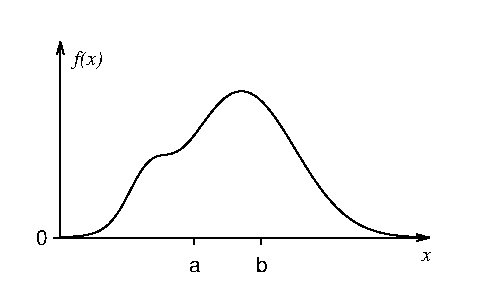
\includegraphics[width=6cm]{probdensity.eps}
    \caption{確率密度関数の例。}\label{fig:probdensity}
\end{figure}

確率密度関数は, 多くの場合, 図\ref{fig:probdensity}のように, 山型のグラフになる(ピークは
ひとつとは限らず, 複数になることもある)。横軸は実現値, 縦軸はその「出やすさ」を表す。
イメージ的には, 図\ref{fig:probdensity_a_b}のように横軸の$a$から$b$の間で, グラフと$x$軸に
挟まれた部分(図で塗りつぶされた部分)の\textgt{面積}が, 「$a$から$b$までの間の実現値が出る確率」
である(それを数式で表現するのが\eref{eq:probdistX1X2}である)。といっても, 縦軸の値
そのものが確率を表すのではないことに注意せよ。なお, 確率は負になることはないので, 確率密度関数
のグラフは$x$軸より下に来ることはない。\\

\begin{figure}[h]
    \centering
    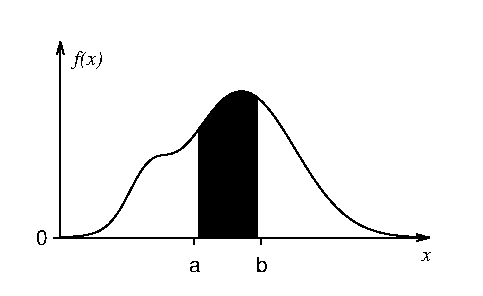
\includegraphics[width=6cm]{probdensity_a_b.eps}
    \caption{黒く塗りつぶされた面積が, \eref{eq:probdistX1X2}, つまり$P(a < X \le b)$に相当する。}\label{fig:probdensity_a_b}
\end{figure}

{\small 注: \eref{eq:defProbDensFunc}や\eref{eq:probdistX1X2}等の
中にある$P()$の中の不等式で, 不等号は$\leq$でも$<$でもよい。例えば
\eref{eq:probdistX1X2}の左辺は, $P(a \le X \le b)$と書いてもよいし, 
$P(a \le X < b)$と書いてもよいし, $P(a < X < b)$と書いてもよい。というのも, 
$<$と$\le$の違いは「その境目にあたる値を含むかどうか」だが, 連続的な
確率変数がそのちょうどぴったりの値をとる確率は, 既に学んだように, 
多くの場合は0であると考えてよい(そうでないような場合もありえるが, それは
高度な数学や確率論になるので今は無視してよい)。従って, 不等号に
等号をつけようがつけまいが, 確率には影響しないのだ。}

さて, いかなる連続的確率変数も, その確率密度関数$f(x)$について
\begin{eqnarray}
\int_{-\infty}^{\infty}f(x)\,dx=1\label{eq:probinteq1}
\end{eqnarray}
である。なぜならば, 上の式の左辺は, $X$が$-\infty$から$\infty$の間の値をとる確率だが, 
そもそも$X$は「$-\infty$から$\infty$の間」以外の値をとりようがないので, これは$X$がとりうる
全ての値についての確率を足し算したものに他ならない。それは全事象に対応するので, 言うまでも
なく1である\footnote{\eref{eq:probinteq1}は, 離散的確率変数に関する
\eref{eq:probsumeq1}を, 連続的確率変数に関して言い換えたものだ。}。


\begin{q}\label{q:stat_clock_sec_densityF} 例\ref{exmpl_clock}で秒針が滑らかに動く場合, 
\begin{enumerate}
\item $X$の確率密度関数$f(x)$を求めよ。ヒント: \eref{eq:probdistX1X2}で$a=0$, $b=60$と考える。
その場合, \eref{eq:probdistX1X2}の左辺はどのような値であるべきだろう? また, 右辺はどのように積分できるだろう?
\item それを用いて, $P(30<X\le30.1)$を求めよ。ヒント: \eref{eq:defProbDensFunc}を使う。$dx=30.1-30=0.1$
\end{enumerate}
\end{q}
\mv

$x$を任意の実数とする。確率変数$X$が, ある値$x$以下であるような確率, 
すなわち$P(X\leq x)$を考える。これは$x$の関数とみなすことができる。
これを\underline{累積分布関数}\index{るいせきぶんぷかんすう@累積分布関数}と
呼ぶ(確率分布関数\index{かくりつぶんぷかんすう@確率分布関数}と呼ぶこともある)。
すなわち, 確率変数$X$の累積分布関数$F(x)$は, 
\begin{eqnarray}F(x):=P(X\leq x)\label{eq:probdist_define}\end{eqnarray}
である(定義)。

\begin{exmpl} サイコロを振って出た目の値$D$は確率変数である。
$x$を任意の実数とする。$D$の累積分布関数$F(x)$は, 以下のような関数である:
\begin{eqnarray}
F(x)=\begin{cases}
0 & x<1\text{のとき}\\
1/6 & 1\leq x<2\text{のとき}\\
2/6 & 2\leq x<3\text{のとき}\\
3/6 & 3\leq x<4\text{のとき}\\
4/6 & 4\leq x<5\text{のとき}\\
5/6 & 5\leq x<6\text{のとき}\\
1 & 6\leq x\text{のとき}\\
\end{cases}
\end{eqnarray}
(例おわり)\end{exmpl}

累積分布関数は, 確率変数が離散的だろうが連続的だろうが, お構いなしに
定義できる。しかし, 確率密度関数は, 離散的な確率変数には定義できず
\footnote{ここでは説明しないが, ディラックのデルタ関数
という, 拡張された関数概念を考えれば, 離散的確率変数にも, 確率密度
関数を定義できる。}, 連続的な確率変数についてのみ, 定義できる。
もし$X$が連続的確率変数なら, 累積分布関数は, 
\eref{eq:probdistX1X2}において$a=-\infty$, $b=x$としたものなので,
\begin{eqnarray}
F(x)=\int_{-\infty}^{x}f(x)\,dx
\label{eq:probdist_infty}\end{eqnarray}
が成り立つ。
\mv

\begin{figure}[h]
    \centering
    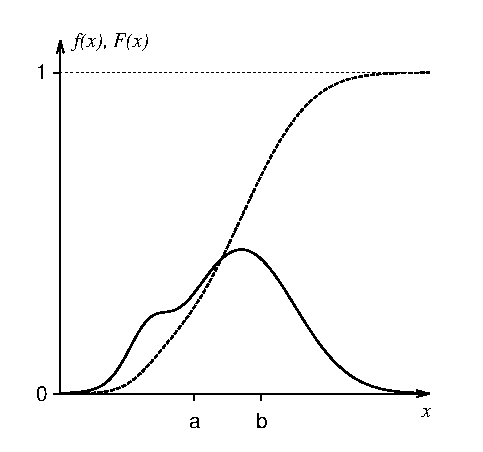
\includegraphics[width=6cm]{probdist.eps}
    \caption{図\ref{fig:probdensity}の確率密度関数$f(x)$ (実線)と, それに対応するの累積分布関数 (太い点線)。}\label{fig:probdist.eps}
\end{figure}

図\ref{fig:probdist.eps}に累積分布関数の例を示す。これは図\ref{fig:probdensity}
で例示した確率密度関数$f(x)$に対応する累積分布関数$F(x)$である。両者の間には,  
\eref{eq:probdist_infty}の関係がある。

\begin{q}\label{q:stat_distF} 連続的確率変数$X$に関する確率密度関数$f(x)$と累積分布関数$F(x)$について, 次式を示せ。
\begin{eqnarray}
\frac{d}{dx}F(x)=f(x)\label{eq:stat_distF_diff}
\end{eqnarray}
\end{q}\mv

\eref{eq:stat_distF_diff}から明らかなように, 連続的確率変数
については, 累積分布関数は確率密度関数の原始関数(のひとつ)であり, 
確率密度関数は累積分布関数の導関数である\footnote{おおざっぱにいえば, 統計データのヒストグラム
が確率密度関数になり, 累積頻度分布が累積分布関数になる。}。

\begin{q}\label{q:stat_distF12} 確率変数(離散的・連続的を問わない)$X$の累積分布関数を
$F(x)$であるとする。$x_1<x_2$として, 次式を示せ:
\begin{eqnarray}
P(x_1 < X \le x_2)=F(x_2)-F(x_1)\label{eq:stat_distF12}
\end{eqnarray}
\end{q}\mv

\eref{eq:stat_distF12}を使えば, 連続的確率変数の確率分布を
表すことができる。つまり, 累積分布関数は, 連続的確率変数の確率分布
の表し方のひとつなのだ。確率分布は実現値と確率の対応関係であり, 
それを「ある値以下になる確率」という形で表すのが累積分布関数である。

\begin{q}\label{q:stat_dist_increase} 任意の確率変数(離散的・連続的を問わない)$X$の
累積分布関数$F(x)$は, 以下の3つの性質を全て満たすことを示せ:
\begin{itemize}
\item 左にいくと($x$が$-\infty$に行くと) 0に近づく。
\item 右に行くと($x$が$\infty$に行くと) 1に近づく。
\item $x$の増加につれて$F(x)$は減少することがない(単調増加関数)。
\end{itemize}
\end{q}

\begin{q}\label{q:stat_clock_accum} 例\ref{q:stat_clock_sec}の累積分布関数を求めよ。\end{q}\mv

\begin{q}\label{q:stat_densityF_distF} 確率密度関数とは何か? 累積分布関数とは何か?\end{q}
\mv

{\small 注: 連続的確率変数の確率分布は, 確率密度関数を使っても表現できるし, 
累積分布関数を使っても表現できる。どちらを使ってもよいのだ。
確率密度関数の方が直感的にはわかりやすいが, 累積分布関数の方が数学的に精密な
理論に適する。}
\vv


\section{連続的確率変数の期待値・分散・標準偏差・共分散・相関係数}

確率変数の期待値とは, 「実現値にその確率を掛けたものの総和」と定義された。これは
離散的確率変数にはOKだが, 連続的確率変数なら, 特定の値をとる確率は0になったり
するので, 具合が悪い。そこで, 連続的確率変数$X$の期待値$E[X]$を, 
\begin{eqnarray}
E[X]:=\int_{-\infty}^{\infty}xf(x)\,dx\label{eq:def_expect_contX}
\end{eqnarray}
と定義しなおす。$f(x)$は, $X$の確率密度関数である。\\

\begin{exmpl}
例\ref{exmpl_clock}の$X$について, その確率密度関数は, 問\ref{q:stat_clock_sec_densityF}で考えた
ように, $0\leq x < 60$で$f(x)=1/60$であり, それ以外で$f(x)=0$である。このとき, 
\begin{eqnarray*}
E[X]=\int_{-\infty}^{\infty}xf(x)\,dx=\int_{0}^{60}\frac{x}{60}dx=\Bigl[\frac{x^2}{120}\Bigr]_{0}^{60}=30
\end{eqnarray*}
となる。これは, 秒針が1秒おきの値を離散的にとる場合の期待値と一致することがわかるだろう。
(例おわり)\end{exmpl}

期待値が定義されれば, あとは離散的確率変数と同じような話が成り立つ。例えば, 
証明は省くが, \eref{eq:stochX_aX_B}, \eref{eq:expect_X_plus_Y}, \eref{eq:expect_Xsum}, 
\eref{eq:expect_X_times_Y}などは連続的確率変数でも成り立つ。

連続的確率変数$X$の分散とは, \peref{eq:defvar}と同様に, 
\begin{eqnarray}
V[X]:=E[(X-\mu)^2]\label{eq:defvarcon}
\end{eqnarray}
と定義する。ここで, $\mu$は, $X$の期待値である。また, \peref{eq:defsd}と同様に, 分散の平方根, すなわち, 
\begin{eqnarray}
\sigma[X]:=\sqrt{V[X]}\label{eq:defssdcon}
\end{eqnarray}
を標準偏差と定義する。

離散的確率変数に関して成り立った多くの定理, すなわち, 
\eref{eq:expect_X_plus_Y}, 
\eref{eq:expect_Xsum}, 
\eref{eq:expect_X_times_Y}, 
\eref{eq:variance_trans_ab}, 
\eref{eq:std_trans_ab}, 
\eref{eq:V_X_Y_2}, 
\eref{eq:V_X_Y_4}, 
\eref{eq:V_X_Y_n}は, 連続的確率変数でも成り立つ(証明は省略する)。また, 
連続的確率変数でも共分散と相関係数を, 離散的確率変数の場合と同じ式
(\eref{eq:def_covar}, \eref{eq:def_corrcoef})で定義する。\\

\begin{exmpl}
連続的に動く秒針が指す値を$X$秒とする。この連続的確率変数$X$の
分散を求めてみよう。既に見たように, $X$の期待値は$\mu=E[X]=30$である。分散は, 
\begin{eqnarray*}
V[X]=E[(X-\mu)^2]=\int_{-\infty}^{\infty}(x-\mu)^2f(x)\,dx\\
=\int_{0}^{60}\frac{(x-30)^2}{60}\,dx=300
\end{eqnarray*}
となる。標準偏差はこの平方根なので, $\sqrt{300}=17.3\cdots$となる。
(例おわり)\end{exmpl}
\mv

\begin{q}\label{q:stat_uniform} $c$を実数, $a$を正の実数とする。確率変数$X$は, $c-a$から$c+a$
の間の値を一様にとり, それ以外の範囲の値をとらないとする\footnote{
この問題は, 「物理学実験1テキスト」P.9の問題3, 4に相当する。}。
\begin{enumerate}
\item $X$の確率密度関数は, $c-a\leq x\leq c+a$で$1/(2a)$, それ以外で0となることを示せ。
\item $E[X]=c$となることを示せ。
\item $V[X]=a^2/3$となることを示せ。
\item $\sigma[X]=a/\sqrt{3}$となることを示せ。
\end{enumerate}\end{q}
\vv


\section{誤差伝播の法則}

以上の話は, 実際の実験や測定で得られたデータの解析に, 非常に役に立つ。

例として, 2つの地点(点Aと点B)の間の距離を巻尺で測ることを考える。この巻尺は少し短すぎて, 
この2地点間をいちどに測ることはできない。そこで, 線分ABの上のどこかに点Cを設定して, 
AC間の距離とCB間の距離をそれぞれ測る。

AC間の距離の真値を$L_{\text{A}}$, CB間の距離の真値を$L_{\text{B}}$とする。AB間の距離の
真値は, 当然, $L_{\text{A}}+L_{\text{B}}$である。ところが, 測定には誤差がつきものなので, 
実際に得られる測定値は, 測定のたびに微妙に違う値になり, それはあらかじめ
予測できるものではない。つまり, 測定値とは, 確率変数なのだ。

いま, AC間の距離の測定値を確率変数$X_{\text{A}}$とし, CB間の距離の測定値を
確率変数$X_{\text{B}}$とする。

もし巻尺の目盛が, 偏った狂い(つまり実際の1$\,$mよりも巻尺の1$\,$mのほうが常に「長すぎ」
もしくは「短すぎ」のようなこと\footnote{このようなことがあれば, 測定値
は常に真値より大きめか小さめの片方に偏った値を出すだろう。そのような誤差を
「系統誤差」と呼ぶ。})が無ければ, $X_{\text{A}}$の期待値は$L_{\text{A}}$, 
$X_{\text{B}}$の期待値は$L_{\text{B}}$に一致するはずだ: 
\begin{eqnarray}
E[X_{\text{A}}]=L_{\text{A}}\label{eq:EXALA}\\
E[X_{\text{B}}]=L_{\text{B}}\label{eq:EXBLB}
\end{eqnarray}

我々は, AB間の距離を, $X_{\text{A}}+X_{\text{B}}$で測定(推定)するのだが, 当然, $X_{\text{A}}+X_{\text{B}}$
も確率変数であり, その期待値は, \eref{eq:expect_Xsum}より
\begin{eqnarray}
E[X_{\text{A}}+X_{\text{B}}]=E[X_{\text{A}}]+E[X_{\text{B}}]=L_{\text{A}}+L_{\text{B}}\nonumber\\
\end{eqnarray}
となり, 実際のAB間に一致するはずだ。

では, これらの測定値の分散や標準偏差はどうなるだろう? 既に述べたように, 
標準偏差は, 確率変数が期待値の周りにどれだけばらつくかの指標である。
つまり, 測定値の標準偏差とは, いわば「誤差」のようなものだ
\footnote{厳密には, これを「不確かさ」と呼び, 「誤差」と区別する。}。では, 
$X_{\text{A}}$に含まれる誤差($X_{\text{A}}$の標準偏差)や$X_{\text{B}}$に含まれる誤差($X_{\text{B}}$の標準偏差)
は, どのようにして$X_{\text{A}}+X_{\text{B}}$の誤差($X_{\text{A}}+X_{\text{B}}$の標準偏差)に効くのか?
それを教えてくれるのが\eref{eq:V_X_Y_4}である。すなわち, 
\begin{eqnarray}
V[X_{\text{A}}+X_{\text{B}}]=V[X_{\text{A}}]+V[X_{\text{B}}]
\end{eqnarray}
である。分散は標準偏差の2乗だから, 
\begin{eqnarray}
(\sigma[X_{\text{A}}+X_{\text{B}}])^2=(\sigma[X_{\text{A}}])^2+(\sigma [X_{\text{B}}])^2\label{eq:gosadenpa04}
\end{eqnarray}
とも書ける。つまり, AB間の誤差の2乗は, AC間の誤差とCB間の誤差のそれぞれの
2乗を足したものだ。誤差そのものが足されるのではなく, 誤差の2乗が
足されるのだ\footnote{これは偶然にも, 三平方の定理に似ている。 
三平方の定理でも, 直角三角形の斜辺の長さと他の2辺の長さに関して, 
長さそのものでなく, 長さの2乗が足されていた。}!

\begin{exmpl}\label{ex:errorpropABBC345}
もし$X_{\text{A}}$の誤差(標準偏差)が3$\,\,$cmで, $X_{\text{B}}$の誤差(標準偏差)が4$\,\,$cmで
あれば, $X_{\text{A}}+X_{\text{B}}$の誤差(標準偏差)は3$\,\,$cm\,+\,4$\,\,$cm\,=\,7$\,$cmなのではなく, 
$\sqrt{(3\,\,\text{cm})^2+(4\,\,\text{cm})^2}=5\,\,\text{cm}$なのだ。(例おわり)
\end{exmpl}

ただし, この話には前提条件が2つある。まず, \eref{eq:EXALA}と\eref{eq:EXBLB}
が成り立たなくてはならない。つまり, 巻尺が偏った狂いを持っていてはならない。
次に, \eref{eq:V_X_Y_4}が成り立つ条件, つまり$X_{\text{A}}$と$X_{\text{B}}$が互いに独立で
なければならない。つまりAC間を測る時とCB間を測る時で, 同じようなミスをしては
ならない\footnote{これらの条件が満たされないならば, 誤差の2乗ではなく, 
誤差の大きさが足されるとみなすべきである。例えば例\ref{ex:errorpropABBC345}
では, AB間の誤差は3$\,$cm+4$\,$cm=7$\,$cmとすべきである。}。

さて, この話は, AB間をもっと多くの区間に分割する場合にも拡張できる。いま, 
AB間を$n$個の区間に分割するとして, 各区間の距離の測定値を$X_1, X_2, \cdots, X_n$
とし, それらは互いに独立であるとする。それらの合計: $Y=X_1+X_2+\cdots+X_n$について, 
\eref{eq:V_X_Y_n}より, 
\begin{eqnarray}V[Y]=V[X_1]+V[X_2]+\cdots+V[X_n]\end{eqnarray}
すなわち, 
\begin{eqnarray}
(\sigma[Y])^2=(\sigma[X_1])^2+(\sigma [X_2])^2+\cdots+(\sigma [X_n])^2\nonumber\\
\label{eq:gosadempa00}
\end{eqnarray}
が成り立つ。すなわち, 以下の定理が成り立つ\footnote{この定理は
慣習的に「法則」と呼ばれているが, 実体は定理である。「伝播」は「でんぱ」と読む。}:
\begin{itembox}{誤差伝播の法則}
複数の測定値の和の誤差(標準偏差)の2乗は, 各測定値の誤差(標準偏差)
の2乗の和になる。ただし, 各測定の\textgt{期待値は真値に一致し}, 各測定どうしは
\textgt{独立でなければならない}。
\end{itembox}
\index{ごさでんぱのほうそく@誤差伝播の法則}
\mv

\begin{q}\label{q:gosadenpa_insuffice} 誤差伝播の法則を述べよ, 
という問に対して, 「複数の測定値の和の誤差(標準偏差)の2乗は, 
各測定値の誤差(標準偏差)の2乗の和になる。ただし, 各測定の
期待値は真値に一致し, 各測定どうしは独立。」と書く人がいる。
これは不正確である。なぜか? どのように修正すればよいか?
\end{q}
\vv

\begin{q}\label{q:error_prop_1m_1km} 
1$\,$kmほどの距離を, 長さ約1$\,$mごとの区間1000個に区切って, ものさし
で測る。ものさしは1$\,$mmごとに目盛が切ってあるので, 1回の
測定(約1$\,$mの測定)の誤差は約1$\,$mmであると考えられる。各区間の
測定値の総和には, どのくらいの誤差が含まれているか?
ただし, 各測定の期待値は真値に一致し, 各測定どうしは独立であるとする。
\end{q}
\vv

実際の現場では, ある量を, 複数の量の測定値から推定する, ということがよく行われる。

\begin{exmpl}\label{exmpl:entoh_Vrh} 例えば, 円筒の体積$V$を測定するには, 底面の半径$r$を
測り(実際は直径を測ってそれを半分にするだろう), 高さ$h$を測って, 
$V=\pi r^2 h$という式で$V$を推定する。(例おわり)\end{exmpl}

このような場合は, 誤差はどのように見積もればよいのだろうか?

今, 最終的に欲しい量$y$が, $y=f(x_1, x_2)$のように, 2つの量$x_1, x_2$の関数である
としよう(上の例では$r$が$x_1$, $h$が$x_2$, $V$が$y$, $\pi r^2h$が$f$に相当する)。
$x_1$の測定値を$X_1=\mu_1+dX_1$と書こう。$\mu_1$は$x_1$の真値であり(従って定数), 
$X_1$と$dX_1$は確率変数である($dX_1$は誤差)。同様に, $x_2$の測定値を$X_2=\mu_2+dX_2$
と書く。$\mu_2$は$x_2$の真値であり(従って定数), $X_2$と$dX_2$は確率変数である
($dX_2$は誤差)。すると, $y$の真値は$f(\mu_1, \mu_2)$であり, $y$の推定値$Y$
は$f(X_1, X_2)$である($Y$も確率変数である)。
ここで, 測定はなかなかうまくいっており, $dX_1$と$dX_2$は小さいとみなせる
としよう。すると, 全微分, すなわち\pref{eq:def_2var_zenbibun}の\eref{eq:def_2var_zenbibun}
を使うことができ,  
\begin{eqnarray}
Y&=&f(X_1, X_2)=f(\mu_1+dX_1,\mu_2+dX_2)\nonumber\\
       &=&f(\mu_1, \mu_2)+ \frac{\partial f}{\partial x_1}\,dX_1+\frac{\partial f}{\partial x_2}\,dX_2\label{eq:gosa_zenbibun02}
\end{eqnarray}
となる。最初と最後で分散をとると, 
\begin{eqnarray}
V[Y] = V\Bigl[f(\mu_1, \mu_2)+ \frac{\partial f}{\partial x_1}\,dX_1+\frac{\partial f}{\partial x_2}\,dX_2\Bigr]\nonumber\\
\label{eq:gosa_zenbibun04}
\end{eqnarray}
となる。$f(\mu_1, \mu_2)$は(未知の量ではあるが)定数なので, \eref{eq:variance_trans_ab}を使うと, 上式の右辺は以下のようになる:
\begin{eqnarray}
 = V\Bigl[\frac{\partial f}{\partial x_1}dX_1+\frac{\partial f}{\partial x_2}dX_2\Bigr]\label{eq:gosa_zenbibun06}
\end{eqnarray}
ここでもし, $\frac{\partial f}{\partial x_1}dX_1$と$\frac{\partial f}{\partial x_2}dX_2$が
互いに独立なら(それぞれの偏微分係数は定数なので, 要するにそれは「$dX_1$と$dX_2$が互いに独立なら」
という条件である), 上の式は, \eref{eq:V_X_Y_4}より, 
\begin{eqnarray}
 = V\Bigl[\frac{\partial f}{\partial x_1}\,dX_1\Bigr]+V\Bigl[\frac{\partial f}{\partial x_2}\,dX_2\Bigr]
\label{eq:gosa_zenbibun07}
\end{eqnarray}
となる。ここで再び\eref{eq:variance_trans_ab}を使うと, \eref{eq:gosa_zenbibun07}は次式のようになる:
\begin{eqnarray}
 = \Bigl(\frac{\partial f}{\partial x_1}\Bigr)^2V[dX_1] + \Bigl(\frac{\partial f}{\partial x_2}\Bigr)^2V[dX_2]
\label{eq:gosa_zenbibun08}
\end{eqnarray}
ところで, また\eref{eq:variance_trans_ab}より, 
\begin{eqnarray}
&&V[X_1]=V[\mu_1+dX_1]=V[dX_1]\\
&&V[X_2]=V[\mu_2+dX_2]=V[dX_2]
\end{eqnarray}
である。これらを使って\eref{eq:gosa_zenbibun08}の$V[dX_1]$と$V[dX_2]$をそれぞれ
$V[X_1]$と$V[X_2]$に書き換え, また, そもそも我々は\eref{eq:gosa_zenbibun04}から出発していたことを思い出すと, 結局, 
\begin{eqnarray}
V[Y] = \Bigl(\frac{\partial f}{\partial x_1}\Bigr)^2V[X_1] + \Bigl(\frac{\partial f}{\partial x_2}\Bigr)^2V[X_2]
\label{eq:gosa_zenbibun12}
\end{eqnarray}
となる。分散は標準偏差の2乗だから, 
\begin{eqnarray}
\sigma_y^2 = \Bigl(\frac{\partial f}{\partial x_1}\Bigr)^2\sigma_1^2 + \Bigl(\frac{\partial f}{\partial x_2}\Bigr)^2\sigma_2^2\label{eq:gosa_zenbibun140}
\end{eqnarray}
となる(ここで, $\sigma[Y]$を$\sigma_y$と書き, $\sigma[X_1]$を$\sigma_1$と書き, $\sigma[X_2]$を$\sigma_2$と書いた)。これは, 
\eref{eq:gosadenpa04}を拡張した式である。

ここでは, $y$が2つの変数$(x_1, x_2)$だけに依存するとしたが, もっとたくさんの変数, すなわち$x_1, x_2, \cdots, x_n$に依存するケースに上の議論を拡張することは容易である(ここではやらないが)。すると, 以下の式が成り立つ:
\begin{eqnarray}
\sigma_y^2 = \Bigl(\frac{\partial f}{\partial x_1}\Bigr)^2\sigma_1^2 + \Bigl(\frac{\partial f}{\partial x_2}\Bigr)^2\sigma_2^2+\cdots+\Bigl(\frac{\partial f}{\partial x_n}\Bigr)^2\sigma_n^2\nonumber\\
\label{eq:gosa_zenbibun14}
\end{eqnarray}

この\eref{eq:gosa_zenbibun14}は, \eref{eq:gosadempa00}を拡張した式である。実際, $y=x_1+x_2+\cdots+x_n$の場合は, 
$\partial f/\partial x_1=\partial f/\partial x_2=\cdots=\partial f/\partial x_n=1$なので, \eref{eq:gosa_zenbibun14}
の中の偏微分係数は全部1になり, \eref{eq:gosadempa00}と同じ式になる。一般には, むしろ
この\eref{eq:gosa_zenbibun14}を誤差伝播の法則という。

例\ref{exmpl:entoh_Vrh}のような状況では, この式を使って, 誤差の大きさを
見積もるのだ。その際, 真値における偏微分係数, すなわち
$\partial f/\partial x_1$, $\partial f/\partial x_2$などを求める
必要があり, そのためには真値, すなわち$\mu_1, \mu_2$などが必要なの
だが, それは実際にはわからない(真値がわかるなら苦労はしない。わからない
から測定するし, 誤差を見積もるのだ)。そこで, これらの偏微分係数
を計算するときは, 真値のかわりに(仕方なく)測定値を入れるのだ。\\

ちなみに「物理学実験1テキスト」P11の式(9)に, これと同じ式が書いてあり, 
「不確かさ伝播の法則」\index{ごさでんぱのほうそく@誤差伝播の法則}
\index{ふたしかさでんぱのほうそく@不確かさ伝播の法則}と称されている。
「誤差」という語は意味がちょっと不明確だという理由で, 最近はかわりに
「\underline{不確かさ}」という語がよく使われる。それはこういう話である:

誤差とは, 「測定値$-$真値」である。上の議論では, $dX_1$や$dX_2$が
誤差である。それは正の値も負の値もとり得る, どのような値なのかは
わからない量である(もしそれがわかる
のなら, 測定値からそれを引くことで真値が得られてしまう。そうできる
のなら苦労はしない)。しかし, それがどのくらいの「大きさ」(絶対値
みたいなもの)かは, なんとなく評価できる, と考えるのだ。それが不確かさ
である。多くの場合は, 不確かさは測定値の標準偏差の推定値で評価され, 
その場合は「標準不確かさ」と呼ばれる。このあたりの詳しい事情は
「物理学実験」で学んで欲しい。\\

\begin{q}\label{q:gosadempa04} 例\ref{exmpl:entoh_Vrh}を考える。
今, ある円筒の体積$V$を推定するために, その半径$r$と高さ$h$を
計測し, $r=35.2$~mm, $h=73.4$~mmという結果を得た。$r$の不確かさは
$\sigma_r=1.0$~mm, $h$の不確かさは$\sigma_h=0.3$~mmであるとして, 
この円筒の体積$V$とその不確かさ$\sigma_V$を見積もれ。\end{q}


\section*{演習問題}

\begin{exq}\label{exq:exp_XY_dep} \eref{eq:expect_X_times_Y}, すなわち, 
\begin{eqnarray*}E[XY]=E[X]E[Y]\end{eqnarray*}
は, $X, Y$が互いに独立な確率変数場合には必ず成り立つ(証明した!)。では, 
確率変数$X, Y$が\textgt{「互いに独立でない」}にもかかわらず, この式が
成り立つような場合はあるだろうか? あるならばその例を挙げよ。無いならば
無いことを証明せよ。\end{exq}

%\begin{q}\label{q:stochastics_English} 以下の言葉を英訳せよ:
%\begin{edaenumerate}<3>
%\item 事象
%\item 背反な
%\item 独立な
%\item 確率
%\item 期待値
%\item 分散
%\item 標準偏差
%\item 確率密度関数
%\item 分布
%\end{edaenumerate}
%\end{q}\mv

\section*{問題の解答}

%
\noindent{\textbf{答}}\ref{q:stat_words0} 
\begin{enumerate}
\item 試行の結果として起きる可能性のあるできごと。
\item 複数の事象の少なくともひとつが起きるという事象。
\item 複数の事象のいずれもが起きるという事象。
\item 何も起きることがないという事象。
\item ある事象に対して「それが起きない」という事象。
\item 他の複数の(空事象でない)事象の和事象と考えることができないような事象。
\item 全ての根元事象の和事象。
\item 複数の事象について, それらが同時に発生することがないこと。
\end{enumerate}
\mv

%
\noindent{\textbf{答}}\ref{q:stat_Pnothing}  たとえ何回試行しても, 空事象$\varnothing$の発生する回数$n(\varnothing)$は0である。
従って, \eref{eq:def_prob_stat}より, $P(\varnothing)=n(\varnothing)/N=0$
\mv

%
\noindent{\textbf{答}}\ref{q:stat_dice2_gt10} 2つのサイコロの出る目の和が
10以上の場合は, $(6,6)(6,5)(6,4)(5,6)(5,5)(4,6)$の6通りで, 2つのサイコロの
出る目のパターンは36通りである。「同様の確からしさの原理」が成り立つとみなして, 
$6/36=1/6$
\mv

\noindent{\textbf{答}}\ref{q:stat_win_lose} (例)「同様の確からしさの原理
は一般的には成り立たない」ということを知らない同僚が, この場面では羨ましい。
\mv

\noindent{\textbf{答}}\ref{q:stat_cond_probability} 略。
ヒント: $P(A\cap B) < P(A|B) < P(B|A)$になるはず。\\


%
\noindent{\textbf{答}}\ref{q:stat_dice_indep_excl} 
\begin{enumerate}
\item サイコロを1回投げて, 1と3は同時に出ることは, 有り得ないので, 排反。また, 1が出たら3が出ることはない, というふうに, 互いへの影響は
大いにあるので, 独立ではない\footnote{従って, 一般に, 排反な事象は互いに独立にはならない。}。
\item 1回めに1, 2回めに3が出ることは, 両方起きる可能性があるから, 排反ではない。また, これらは互いに影響を与えないので, 独立。
\item 4が出たら$A, B$両方の事象が起きたことになるので, 排反ではない。偶数が出るならば, その場合, 目は2, 4, 6のうちどれかなので, 
4が出る確率は大きくなる。従って, 独立でもない。
\end{enumerate}
\mv

%
\noindent{\textbf{答}}\ref{q:stat_coin10}  $(1/2)^{10}=1/1024$
\mv

% コインを5回投げたとき, 表が3回出る確率は?
\noindent{\textbf{答}}\ref{q:stat_5_3coins} $B(5, 1/2)$
に従う確率変数$X$について, $P(X=3)$を求めればよい。
\eref{eq:stoch_dist_Bernoulli08}より, 
$P(X=3)\,=\,_5\text{C}_3\,(1/2)^3(1-1/2)^{5-3}\,=\,_5\text{C}_3(1/2)^5=10/32=5/16$。
\mv

% 5枚のコインを同時に投げたとき, 表が3枚出る確率は?
\noindent{\textbf{答}}\ref{q:stat_5_3coins2} 問\ref{q:stat_5_3coins}と同じで, 5/16。
\mv

\noindent{\textbf{答}}\ref{q:stat_defexp1} 略。がんばれ!
\mv

\noindent{\textbf{答}}\ref{q:stat_defexp2} 略。
\mv

%
\noindent{\textbf{答}}\ref{q:stat_coin_sq}  各目の出る確率はいずれも$1/6$なので, \
\begin{eqnarray*}
\frac{1^2}{6} + \frac{2^2}{6} + \frac{3^2}{6} + \frac{4^2}{6} + \frac{5^2}{6} + \frac{6^2}{6} = \frac{91}{6} \fallingdotseq 15.2
\end{eqnarray*}
\mv

% ベルヌーイ分布$B(n, p)$に従う確率変数
\noindent{\textbf{答}}\ref{q:stat_Bernoulli}
\begin{eqnarray*}
E[X]=1\times P(X=1)+0\times P(X=0)=P(X=1)=p
\end{eqnarray*}
\mv

\noindent{\textbf{答}}\ref{q:stat_expect_X_plus_Y} 略。
\mv

%
\noindent{\textbf{答}}\ref{q:stat_3coins}  表が$k$回出る確率を$P(k)$とすると, $P(0)=1/8$, $P(1)=3/8$, $P(2)=3/8$, $P(3)=1/8$である。賞金額の期待値は, $0\times P(0)+100\times P(1)+200\times P(2)+300\times P(3)=1200/8=150\text{円}$。
\mv


% 2項分布$B(n, p)$に従う確率変数$X$について, 次式を示せ:
\noindent{\textbf{答}}\ref{q:stat_binomial_exp} 
$k$回目のベルヌーイ試行で事象が起きる回数(0か1)を確率変数$X_k$で表す($k$は
1以上$n$以下の任意の整数)。すると, $X=X_1+X_2+\cdots+X_n$と
表される。従って, 
\begin{eqnarray}
E[X]&=&E[X_1+X_2+\cdots+X_n]\nonumber\\
&=&E[X_1]+E[X_2]+\cdots+E[X_n]\label{q:stat_binomial_exp_ans8}
\end{eqnarray}
となる(\eref{eq:expect_Xsum}を使った)。ここで, $X_1, X_2, \cdots, X_n$は
同一のベルヌーイ分布に従う確率変数なので, \pref{q:stat_Bernoulli_E}の
\eref{q:stat_Bernoulli_E}より{\small (注: \eref{q:stat_Bernoulli_E}の$X$はここでは
$X_1, X_2, \cdots, X_n$のこと!)}, 
\begin{eqnarray}
E[X_1]=E[X_2]=\cdots=E[X_n]=p\label{q:stat_binomial_exp_ans4}
\end{eqnarray}
従って, \eref{q:stat_binomial_exp_ans8}は$np$となる。\qed
\mv

\noindent{\textbf{答}}\ref{q:stat_expect_X_times_Y} 略。
\mv

%
\noindent{\textbf{答}}\ref{q:stat_2coins_indep} 
\begin{enumerate}
\item
$P(X=0, Y=0)=1/4$,\\
$P(X=100, Y=0)=0$,\\
$P(X=0, Y=100)=1/4$,\\
$P(X=100, Y=100)=1/2$ である。従って, 
\begin{eqnarray*}E[X+Y]=0\times\frac{1}{4}+100\times(0+\frac{1}{4})+200\times\frac{1}{2}=125\end{eqnarray*}
一方, 例より$E[X]=50$, $E[Y]=75$だったから, 
\begin{eqnarray*}E[X]+E[Y]=50+75=125\end{eqnarray*}
従って与式が成り立つ。
\item このルールを廃止したら, 
\begin{eqnarray*}
&&P(X=0, Y=0)=P(X=100, Y=0)\\
&&=P(X=0, Y=100)=P(X=100, Y=100)=\frac{1}{4}
\end{eqnarray*}
である。従って, 
\begin{eqnarray*}
&&P(XY=10000)=P(X=100, Y=100)=\frac{1}{4}\\
&&P(XY=0)=1-P(XY=10000)=1-\frac{1}{4}=\frac{3}{4}
\end{eqnarray*}
従って, 
\begin{eqnarray*}E[XY]=0\times\frac{3}{4}+10000\times\frac{1}{4}=2500\end{eqnarray*}
一方, $E[X]=E[Y]=50$なので, $E[X]E[Y]=2500$。従って与式が成り立つ。\qed
\end{enumerate}
\mv

%
\noindent{\textbf{答}}\ref{q:stat_EVS_dim} 
\begin{enumerate}
\item 実現値(資源生の靴のサイズとしてあり得る値)を$x_1, x_2, \cdots, x_n$とする。
資源生の人数を$M$とし, 靴のサイズが$x_k$の資源生の人数を$m_k$とする。
どの資源生も同じ確からしさで選ばれるとみなせば, 靴のサイズ$x_k$の
資源生が選び出される確率は, \eref{eq:def_prob_math}より, 
$m_k/M$である。従って, $P(X=x_k)=m_k/M$となる。これは人数/人数なので, 
無次元。同様に考えれば, 全ての$k$について, $P(X=x_k)$は無次元である。
つまり, 確率は無次元。
\item \eref{eq:def_expectation0}をこの問題に適用して考える。確率は無次元なので, 
\eref{eq:def_expectation0}の右辺の次元は, 実現値$x_k$の次元である。
従って, 期待値の次元は実現値の次元に等しい。つまり「長さ」である。
\item 期待値を$\mu$と書く。\eref{eq:defvar}をこの問題に適用して考える。この式は, 
\begin{eqnarray*}
V[X]=E[(X-\mu)^2]=\sum_{k=1}^{n}(x_k-\mu)^2P(X=x_k)
\end{eqnarray*}
と書ける($\mu=E[X]$)。最右辺の次元は, (2)と同様に考えて, $(x_k-\mu)^2$の次元, つまり
実現値の2乗の次元である。従って, 分散の次元は, 実現値の2乗の次元, つまり
「長さの2乗」である。
\item 標準偏差は分散の平方根なので, その次元は分散の次元の1/2乗である。
分散の次元は, 実現値の2乗の次元に等しいので, 標準偏差の次元は実現値の次元, 
つまり, 「長さ」である。
\end{enumerate}

%
\noindent{\textbf{答}}\ref{q:stat_3coins_var}  問\ref{q:stat_3coins}より, 賞金額の期待値は150円。賞金額の分散は, 
\begin{eqnarray*}
&&(0\text{円}-150\text{円})^2\times P(0)+(100\text{円}-150\text{円})^2\times P(1)\\
+&&(200\text{円}-150\text{円})^2\times P(2)+(300\text{円}-150\text{円})^2\times P(3)\\
=&&7500\text{円}^2
\end{eqnarray*}
従って, 標準偏差は, $\sqrt{7500}\text{ 円}\fallingdotseq87\text{ 円}$。

別解: 100円玉1枚を投げて表が出たらもらえる, という確率変数の分散は
\begin{eqnarray*}
&&(0\text{円}-50\text{円})^2\times\frac{1}{2}+(100\text{円}-50\text{円})^2\times\frac{1}{2}\\
&&=2500\text{円}^2
\end{eqnarray*}
3枚の100円玉を投げるのは互いに独立なので, これらの和の分散は, 1枚の分散3つの和。従って, $2500\times3=7500\text{円}^2$。
注: ここで分散の値に単位として円$^2$とつけたが, この「2乗」は必要である。
\mv

%\eref{eq:stoch_dist_Bernoulli}で示したベルヌーイ分布に従う確率変数$X$について, 次式を示せ:
\noindent{\textbf{答}}\ref{q:stat_Bernoulli_V} \eref{q:stat_Bernoulli_E}より$E[X]=p$
である。これを$\mu$と置くと, 
\begin{eqnarray*}
V[X]&=&E[(X-\mu)^2]=E[(X-p)^2]\nonumber\\
    &=&(1-p)^2p+(0-p)^2(1-p)\nonumber\\
    &=&p(1-p)^2+p^2(1-p)\nonumber\\
    &=&p(1-p)(1-p+p)=p(1-p)
\end{eqnarray*}
\mv

%2項分布$B(n, p)$に従う確率変数$X$について, 次式を示せ:
\noindent{\textbf{答}}\ref{q:stat_binomial_V} \eref{eq:binom_Bernoulli_sum}
より, 
\begin{eqnarray}
V[X]=V[X_1+X_2+\cdots+X_n]\label{eq:stat_binomial_V_ans2}
\end{eqnarray}
である。ここで, $X_1, X_2, \cdots, X_n$は互いに独立なので, 
\eref{eq:V_X_Y_n}を使って, 
\begin{eqnarray}
V[X]=V[X_1]+V[X_2]+\cdots+V[X_n]\label{eq:stat_binomial_V_ans4}
\end{eqnarray}
とできる。ところで, $X_1, X_2, \cdots, X_n$は同一のベルヌーイ分布に従う
ことと, \eref{eq:stat_Bernoulli_V}より, 
\begin{eqnarray}
V[X_1]=V[X_2]=\cdots=V[X_n]=p(1-p)\nonumber\\\label{eq:stat_binomial_V_ans6}
\end{eqnarray}
である。\eref{eq:stat_binomial_V_ans6}を\eref{eq:stat_binomial_V_ans4}に
代入して, 
\begin{eqnarray*}
V[X]&=&p(1-p)+p(1-p)+\cdots+p(1-p)\\
    &=&np(1-p)
\end{eqnarray*}
となり, 与式を得る。\qed
\mv

\noindent{\textbf{答}}\ref{q:stat_clock_sec} 
(1) $X$は60個の整数値のいずれも同じ確からしさでとりえるので, 30に限らず, 
ひとつの特定の値をとる確率は, 1/60。(2) $X$は0から59.9までの600個の値
のいずれも同じ確からしさでとりえるので, 30に限らず, ひとつの特定の値をとる確率は, 
1/600。(3) 同様に考えて, 1/6000。 (4) 同様に考えて, $1/(60\times10^n)$。
(5) 「滑らかに動く」とは, 限りなく小さな刻みで動くことと考え, 
(4)で$n\rightarrow\infty$を考えると, $1/(60\times10^n)\rightarrow0$。
したがって, 0。
\mv

% 次式を示せ: P(a < X \le b)=\int_{a}^{b}f(x)\,dx
\noindent{\textbf{答}}\ref{q:stat_densityF}  $a$から$b$の範囲を, $n$個の微小区間に分割する。すなわち, 
$a=x_0<x_1<x_2<\cdots< x_n=b$とする。また, $0\le k< n$として, 
$\Delta x_k=x_{k+1}-x_k$とする。\eref{eq:defProbDensFunc}より, 
\begin{eqnarray}P(x_k<X\le x_{k+1})\fallingdotseq f(x_k)\Delta x_k\end{eqnarray}
である。従って, 
\begin{eqnarray}P(a<X\le b)&=&\sum_{k=0}^{n-1}P(x_k<X\le x_{k+1})\nonumber\\
&\fallingdotseq&\sum_{k=0}^{n-1}f(x_k)\Delta x_k\end{eqnarray}
$\Delta x_k\rightarrow 0$, $n\rightarrow \infty$とすれば, 
積分の定義より, 与式の右辺に一致する。
\mv

% 時計の秒針が指す値を確率変数
\noindent{\textbf{答}}\ref{q:stat_clock_sec_densityF} (略解) 
(1) $f(x)=1/60$ ... そうなる理由も述べること! (2) 
$P(30<x\le30.1)=f(30)\times(30.1-30.0)=(1/60)\times0.1=1/600$
\mv

% 次式を示せ: \frac{d}{dx}F(x)=f(x)
\noindent{\textbf{答}}\ref{q:stat_distF}  導関数の定義(\peref{eq:define_dif2})より, 
\begin{eqnarray*}\frac{d}{dx}F(x)=\lim_{\Delta x\rightarrow 0}\frac{F(x+\Delta x)-F(x)}{\Delta x}\end{eqnarray*}
ここで\eref{eq:probdist_infty}より, 右辺は, 
\begin{eqnarray*}\lim_{\Delta x\rightarrow 0}\frac{\int_{-\infty}^{x+\Delta x}f(x)dx-\int_{-\infty}^{x}f(x)dx}{\Delta x}\\
=\lim_{\Delta x\rightarrow 0}\frac{\int_{x}^{x+\Delta x}f(x)dx}{\Delta x}\end{eqnarray*}
ところで, $\Delta x$が十分に小さければ, $x$から$x+\Delta x$の間で$f(x)$はほとんど一定とみなせるから, 上の式は, 積分の公式6より, 
\begin{eqnarray*}
=\lim_{\Delta x\rightarrow 0}\frac{f(x)\int_{x}^{x+\Delta x}dx}{\Delta x}
=\lim_{\Delta x\rightarrow 0}\frac{f(x)\Delta x}{\Delta x}=f(x)\end{eqnarray*}
となる。
\mv

% 確率密度関数とは何か? 累積分布関数とは何か?
\noindent{\textbf{答}}\ref{q:stat_densityF_distF}  
確率変数$X$, 微小量$dx$について, $P(x<X\le x+dx)=f(x)dx$となるような
関数$f(x)$のことを$X$の確率密度関数という。また, $P(X\leq x)$を$x$の
関数とみなしたものを, $X$の累積分布関数という。
\mv

% 次式を示せ: P(x_1 < X \le x_2)=F(x_2)-F(x_1)
\noindent{\textbf{答}}\ref{q:stat_distF12}  累積分布関数の定義より, 次式が成り立つ:
\begin{eqnarray*}&&F(x_2)-F(x_1)\\
&&=\int_{-\infty}^{x_2}f(x)dx-\int_{-\infty}^{x_1}f(x)dx=\int_{x_1}^{x_2}f(x)dx\end{eqnarray*}
\eref{eq:probdistX1X2}より, これは$P(x_1<X\leq x_2)$に等しい。
\mv

% 一様分布の確率密度関数・分散・標準偏差
\noindent{\textbf{答}}\ref{q:stat_uniform}  
(1) $X$は$c-a\leq x\leq c+a$で一様な確率で値をとるので, $X$の確率密度関数$f(x)$は, 
$c-a\leq x\leq c+a$で, 一定値をとる。それを$A$とする。また, $c-a\leq x\leq c+a$以外の範囲
には$X$は値をとらないから, $c-a\leq x\leq c+a$以外の範囲では$f(x)=0$である。さて, 
\begin{eqnarray*}
\int_{-\infty}^{\infty}f(x)dx=\int_{-\infty}^{c-a}f(x)dx+\int_{c-a}^{c+a}f(x)dx\\
+\int_{c+a}^{\infty}f(x)dx=\int_{c-a}^{c+a}A\,dx=2Aa
\end{eqnarray*}
となる。\eref{eq:probinteq1}より, $2Aa=1$。従って, $A=1/(2a)$である。
\begin{eqnarray*}
&&\text{(2) }\,\,\,E[X]=\int_{c-a}^{c+a}\frac{x\,dx}{2a}=\Bigl[\frac{x^2}{4a}\Bigr]_{c-a}^{c+a}=c\\
&&\text{(3) }\,\,\,V[X]=\int_{c-a}^{c+a}\frac{(x-c)^2\,dx}{2a}=\Bigl[\frac{(x-c)^3}{6a}\Bigr]_{c-a}^{c+a}=\frac{a^2}{3}\\
&&\text{(4) }\,\,\,\sigma[X]=\sqrt{V[X]}=\frac{a}{\sqrt{3}}
\end{eqnarray*}
\mv

\noindent{\textbf{答}}\ref{q:gosadenpa_insuffice} 不正確な
ポイントは2つある。まず, 「誤差(標準偏差)の和の2乗」の部分は
「和の誤差(標準偏差)の2乗」としなければならない。これらは
必ずしも一致しない。次に, 末尾は「でなければならない。」とか, 
「であることが必要。」とまで書かねばならない。これが
無いと, 「各測定の期待値は真値に一致し, 各測定どうしは独立」
ということが定理の成立条件でなく定理の結論の一部であると
誤解される可能性がある。
\vv


%
\noindent{\textbf{答}}\ref{q:error_prop_1m_1km}
各区間の測定値を$X_1, X_2, \cdots, X_{1000}$とする。
その総和を$Y=X_1+X_2+ \cdots +X_{1000}$とする。
各区間の測定値の標準偏差を1 mmとすると, 
$V[X_1]=V[X_2]=\cdots=V[X_{1000}]=(1\,\,\text{mm})^2$
である。従って, 誤差伝播の法則より, $V[Y]=V[X_1]+V[X_2]+\cdots+V[X_{1000}]
=1000\times(1\,\,\text{mm})^2=1000\,\,\text{mm}^2$。
従って, $\sigma[Y]=\sqrt{V[Y]}=\sqrt{1000\,\,\text{mm}^2}\fallingdotseq 32\,\,\text{mm}$, 
すなわち, 約3 cmの誤差が含まれていると考えられる。
\mv

\noindent{\textbf{答}}\ref{q:gosadempa04} \eref{eq:gosa_zenbibun14}で$n=2$, $x_1=r$, $x_2=h$, $\sigma_1=\sigma_r$, $\sigma_2=\sigma_h$, $\sigma_y=\sigma_V$と置き換えれば, 
\begin{eqnarray*}
\sigma_V^2 = \Bigl(\frac{\partial f}{\partial r}\Bigr)^2\sigma_r^2 + \Bigl(\frac{\partial f}{\partial h}\Bigr)^2\sigma_h^2
\end{eqnarray*}
となる。$f=\pi r^2h$なので, $\frac{\partial f}{\partial r}=2\pi r h$, $\frac{\partial f}{\partial h}=\pi r^2$である。従って, 
\begin{eqnarray*}
&&\sigma_V^2 = (2\pi r h)^2 \sigma_r^2 + (\pi r^2)^2\sigma_h^2\quad\text{従って, }\\
&&\sigma_V = \sqrt{(2\pi r h)^2 \sigma_r^2 + (\pi r^2)^2\sigma_h^2}
\end{eqnarray*}
となる。この右辺に与えられた値を代入すると, \\
$V=285713.8\cdots$~mm$^3$, $\sigma_V=16275.6\cdots$~mm$^3$\\
となる。$\sigma_V$の有効数字を2桁とすると, \\
$\sigma_V=16000$~mm$^3$
となる。$V$の有効数字がこの2桁(1と6; $10^4$と$10^3$の桁)を含む
ように, $10^2$の桁(7という数字)を四捨五入で丸めると, 
$V=286000$~mm$^3$となる。すなわち, 
$V=(2.86\pm 0.16)\times10^5$~mm$^3$。
\hv

\section*{コラム: 覚えることと理解すること}

本章と次章(確率論・統計学)は, 耳慣れない言葉がたくさん出てきて, 
その定義を覚えるのが大変だ。そういうとき, 数学が得意な
学生は, 「数学は理解すれば自然に覚えられるものだ。理解せず
に覚えるなんて無意味だ!」と思ってしまい, ひとつひとつの言葉
に素直に向き合えずに, 挫折してしまいがちだ。

もちろん, 数学は理解しなければ無意味。でも, 大学の数学
は抽象的なものが多く, すぐに理解できるようなものはわずかなのだ。

そこで威力を発揮するのは, 数学好きの人が毛嫌いする「理解できなくてもまず覚える」
というアプローチだ。定義を呪文のように覚えるのだ。数学は全て定義(公理)
から組み立てられるので, 定義が頭に入ってれば, あとは丁寧に論理を
たどれば, 教科書や授業の話にくらいついていける。そうしているうちに, 
その「意味」が徐々にわかってくる。要するに, 「覚えてから理解する」のだ。

なぜこんな不自然なアプローチをするのだろうか? 喩え話で考えてみよう。

君が料理を習うとき, まず指示に従って食材を揃える。
そのとき君は, 個々の食材がなぜ必要なのか知りたいだろう。
しかし, 普通はそんなことは説明されない。それよりも, その食材を使って
料理が完成するまでの過程を君は体験させられるだろう。それを何回も
繰り返し, いろいろ試す中で, 個々の食材や調味料がどのような
役割をしているのかを, 君は理解するのだ。\mv

こういうことは, 他にも多くの学びごとにもある。
スポーツも楽器演奏も, 陶芸や木工のような工芸も, 野菜作りや米作りのよう
な農作業もそうだ。規則や道具や材料や練習メニューや作業工程といった
個々の要素の「意味」は最初に説明されたりしないし, たとえ説明されても
わかることは少ないだろう。とにかくやってみて, ある程度習得した後
になってわかるのだ。なぜだろう? 簡単なことだ。個々の要素は全体の中
で役割を担うのだから, 全体像が見えないと個々の役割, すなわち
「意味」は見えないのだ。

確率論・統計学も同じだ。確率変数や期待値, 分散, 確率分布, 独立
などの概念は, 確率論・統計学を明快な理論体系に組み上げるための材料
だ。それらの本当の意味や役割は, 確率論・統計学の全体像が見えて
こないとわからない。しかし, その全体像は, これらの言葉を使わない
と見えて来ないのだ。ここに数学を学ぶ時の矛盾がある。\mv

「理解する」とか「意味を考える」ことが無意味だと言っている
のではない。それらはとても大切なプロセスだ。ただ, 数学に
おいて, 学ぶことの最初の段階からそれらを過剰に求めることは, 
むしろ有害で, かえって理解や意味を遠ざけてしまうのだ。

ならば闇雲に覚えればいいのかというと, そうでもない。数学は
体系性が重要である。定義を覚えるときは, その定義に出てくる
ひとつひとつの言葉の定義がわかっていなくてはならない。
「定義全体の意味」は当面はわからなくてもいいが, 定義に出てくる
「個々の言葉の意味」はわかっていなくてはならない。

